{

\pagestyle{fancy}

\pagestyle{fancy}
\fancyhead{}


\hypersetup{linkcolor=black}

\lhead{Table des matières}

% Table of contents -------------------------------------------------
\tableofcontents\thispagestyle{fancy}
\listoffigures
\listoftables

% Chapter 1 Introduction ---------------------------------------------------------
% -------------------------------------------------------------------
\pagebreak
\lhead{Introduction}
\chapter{Introduction}\thispagestyle{fancy}


\section{Présentation du projet}
Notre projet consiste à construire des lunettes intelligentes pour les gens malvoyants. Les services qu'on veut offrir à travers ce produit sont les trois suivants:
\begin{itemize}
    \item Reconnaissance faciale.
    \item Détection d'objets.
    \item Prédiction de texte.
\end{itemize}

\begin{figure}[H] 
\centering
{\adjincludegraphics[width=15cm, height=6cm,clip]{4-Images/3-services.PNG}}\\[0.5cm]
\caption{Les trois services}
\label{fig:figure17}
\end{figure}

Nous voulons donc construire des lunettes intelligentes qui utilisent l'intelligence artificielle (IA) pour extraire des informations des images et dire verbalement à celui qui les porte ce qu'il regarde.

\subsection{La problématique}

Toutes les lunettes intelligentes sont basées sur une carte électronique qui prend les images en entrée et en indique le contenu en sortie. Si nous voulons offrir des services de haute qualité, nous devons construire des \textbf{modèles IA} capables de prédire le contenu d'une image avec une grande confiance dans un court laps de temps. Un modèle haute performance a une architecture complexe qui prend l'image en entrée et effectue un \textbf{million d'opérations} et donne le résultat. Si nous voulons également le faire en peu de temps, nous devons disposer d'une ressource de calcul, qui est trop chère capable d'effectuer des opérations rapidement. Si on veut faire tourner un modèle dans une carte \textbf{Arduino} par exemple, cette carte va \textbf{chauffer} au bout d'un certain temps et \textbf{planter}. Donc nous sommes devant deux cas :
\begin{itemize}
    \item Utiliser un équipement peu performant à bas prix.
    \item Utiliser un équipement performant à prix élevé.
\end{itemize}

Les grandes entreprises qui veulent proposer des lunettes intelligentes hautes performances utilisent des \textbf{cartes électroniques spéciales} qui rendent leurs produits si chers, on parle de \textbf{milliers d'euros}. Nous voulons, à travers ce projet, construire des lunettes intelligentes à faible coût et performantes. Nous détaillerons la solution dans la section suivante

\subsection{Solution retenue}
Notre solution est de construire des lunettes intelligentes qui s'appuient sur un serveur où le traitement d'image ou de vidéo se fera rapidement. Cette solution couvre également le cas où il n'y a pas de connexion internet entre nos lunettes et le serveur. Un serveur est censé fonctionner en continu et offrir des services en peu de temps. Il peut prendre une grande quantité de données et les traiter rapidement et donner le résultat. Cette solution va nous permettre d'avoir un produit à faible coût, car allouer une machine dans un serveur revient beaucoup moins cher que d'utiliser une carte électronique onéreuse.

Nous aurons toujours besoin d'utiliser une carte électronique pour deux raisons :

\begin{itemize}
    \item Envoyez les données au serveur,en cas d'une connexion internet, où il existe des modèles IA de haute performance qui peut prédire le contenu de l'image avec de hautes performances.
    \item Traiter les données avec un modèle IA qui ne conduira pas la carte électronique à chauffer.
\end{itemize}

Notre solution est celle présentée dans l'image suivante :
\begin{center}
\begin{figure}[H] 
\centering
{\adjincludegraphics[width=12cm, height=4cm,clip]{4-Images/client-server.PNG}}\\[0.5cm]
\caption{Client-Serveur}
\label{fig:figure1}
\end{figure}
\end{center}
%{flushleft} : prevent section header from taking being centered when the section in center tag

\section{État de l'art}

De nombreuses entreprises ont créé des lunettes intelligentes pour les malvoyants il y a quelques années et améliorent leurs produits au fil du temps. Ils existent beacuoup des appareils permettant d'aider les aveugles et les malvoyants à percevoir leur environnement avec quelques fonctionnalités différentes d'un appareil à l'autre.
Au début, les lunettes intelligentes étaient des appareils simples fournissant des services  basique. De plus en plus, elles deviennent plus performants et offrent plusieurs fonctionnalités. Dans le tableau suivant, nous allons des lunettes intelligentes et comparé leurs caractéristiques aux nôtres : \\[0.5cm]


% [h] means place the table here and not at the top
% add space bewteen rows by 1.4 factor
% website : https://tex.stackexchange.com/questions/195387/table-out-of-margin-any-suggestion

\renewcommand{\arraystretch}{1.4}

\begin{table}[h!]
{
\centering
% \begin{adjustbox}{max width=1.1\textwidth,center} for centering table and prevent it from going out of margin
\begin{adjustbox}{max width=1.1\textwidth,center}
\begin{tabular}{| c | c | c | c | c |} 
 \hline
 % |c| : vline in left and right
\multicolumn{1}{|c|}{\diagbox{\textbf{Fonctions}}{\textbf{Produits}}} &  \textbf{Oton Glass} & \textbf{Eyesynth-Smart} & \textbf{Google Glass} & \textbf{Notre produit} \\ [0.5ex] 
 \hline
 Conversion image en son & 
 \cellcolor[HTML]{ff7373}\textbf{Non} &  \cellcolor[HTML]{73ffa6}\textbf{Oui} & \cellcolor[HTML]{73ffa6}\textbf{Oui} &  \cellcolor[HTML]{73ffa6}\textbf{Oui} \\ 
 
 
 Conversion texte en son  & \cellcolor[HTML]{73ffa6}\textbf{Oui}&   
 \cellcolor[HTML]{ff7373}\textbf{Non}& \cellcolor[HTML]{73ffa6}\textbf{Oui}&  \cellcolor[HTML]{73ffa6}\textbf{Oui} \\ 
 
 
 Reconnaissance faciale & 
 \cellcolor[HTML]{ff7373}\textbf{Non}&   
 \cellcolor[HTML]{ff7373}\textbf{Non}& \cellcolor[HTML]{73ffa6}\textbf{Oui}&  \cellcolor[HTML]{73ffa6}\textbf{Oui} \\ 
 
 
 La traduction & 
 \cellcolor[HTML]{ff7373}\textbf{2 langues}&   
 \cellcolor[HTML]{ff7373}\textbf{Non}& \cellcolor[HTML]{73ffa6}\textbf{Oui}&  \cellcolor[HTML]{73ffa6}\textbf{Oui} \\
 
 
 Ressources puissantes& 
 \cellcolor[HTML]{ff7373}\textbf{Non}&   
 \cellcolor[HTML]{ff7373}\textbf{Non}& \cellcolor[HTML]{73ffa6}\textbf{Oui}&  \cellcolor[HTML]{73ffa6}\textbf{Oui} \\
 
 
Avoir un coût raisonnable& 
 \cellcolor[HTML]{73ffa6}\textbf{Oui}&   
 \cellcolor[HTML]{ff7373}\textbf{Non}& \cellcolor[HTML]{ff7373}\textbf{Non}&  \cellcolor[HTML]{73ffa6}\textbf{Oui} \\ [1ex]
 
 

 \hline
\end{tabular}
\end{adjustbox}
}
\caption{Fonctions disponibles}
\label{table:1}
\end{table}



Bien que notre produit propose également de nombreuses fonctions, il va sûrement, comme évoqué plus précédemment, être confronté à de nombreux appareils concurrents, il a donc fallu réfléchir à comment arriver à un appareil plus performant.

Grâce au concept de cloudification, en utilisant les ressources d'un Cloud ou d'un serveur, on peut éviter d'utiliser des microcontrôleurs très puissants, comme l'ont fait de nombreuses lunettes, et proposer des lunettes intelligentes abordables pour tous.

Comme cité précédemment, nos lunettes fonctionneront lorsqu'il y aura un réseau Internet et nous aurons des modèles de prédiction puissants qui ne peuvent pas fonctionner sur raspberry pi pendant longtemps sans chauffer la carte. Lorsqu'il n'y a pas de connexion Internet, le raspberry pi exécutera différents modèles de prédiction qui ne conduiront pas à un échauffement de la carte.





% Chapter 2 Raspberry PI ---------------------------------------------------------
% -------------------------------------------------------------------

\pagebreak
\lhead{Raspberry PI}

\chapter{Raspberry PI}\thispagestyle{fancy} % ----------
Pour notre projet, Nous avons choisi Raspberry PI comme la électronique carte de base. De plus, ce composant est également capable d'effectuer un traitement local lorsqu'il n'y a pas de connexion internet vers serveur.
\section{Modèle PI4}

% Remove top margin of wrapped fifure : https://tex.stackexchange.com/questions/160585/how-can-i-reduce-top-margin-of-wrapfigure : \raisebox{0pt}[\dimexpr\height-0\baselineskip\relax]
% [9] : wrapping 9 lines
\begin{wrapfigure}[9]{R}[1.5cm]{0.6\textwidth}
\centering
\raisebox{0pt}[\dimexpr\height-1.8\baselineskip\relax]{\adjincludegraphics[width=7cm, height=6cm,clip]{4-Images/rasp4.PNG}}
\caption{Raspberry PI 4}
\label{fig:figure3}
\end{wrapfigure} 
Au cours de nos recherches, nous avons choisi
le modèle Raspberry Pi 4 en raison de la disponibilité d'une antenne Wi-Fi et Bluetooth. Avec ce modèle, nous voulons effectuer un traitement local. Dans tous les cas, l'utilisateur voudra entendre le résultat du traitement avec des écouteurs bluetooth pour garantir la protection de la vie privée des utilisateurs.\\[1cm]

%\begin{figure}[H] 
%\centering
%\frame{\adjincludegraphics[width=12cm, %height=8cm,clip]{4-Images/rasp4.PNG}}\\[0.5cm]
%\caption{Raspberry PI 4}
%\label{fig:figure1}
%\end{figure}

\section{Autres composantes}
Il y a d'autres équipements qui seront liés à notre Raspberry Pi que nous allons détailler ensuite.
    \subsection{Module Caméra}
    \begin{wrapfigure}[8]{r}[1.5cm]{0.4\textwidth}
    \centering
    \raisebox{0pt}[\dimexpr\height-1.8\baselineskip\relax]{\adjincludegraphics[width=4cm, height=3cm,clip]{4-Images/pi-camera.PNG}}
    \caption{Caméra rev2}
    \label{fig:figure3}
    \end{wrapfigure} 
    Nous aurons besoin d'une caméra compatible qui répond le mieux à nos besoins.

    Le modèle choisi : Caméra Raspberry PI Rev 2.1 avec 8 mégapixels et 30fps  qui donne le meilleur rapport Qualité/Prix.
    
    Le Raspberry Pi possède deux connecteurs particuliers : les ports DSI - Display Serial Interface et CSI -Camera Serial Interface. Ils permettent respectivement de relier un écran et une caméra au Raspberry Pi. Nous utiliserons donc  le port CSI dans le but de capturer des photos et des vidéos. Le branchement de la caméra avec le Raspberry Pi est donc très simple.
    On peut vérifier que la caméra est détecté :
    \begin{figure}[H] 
    \centering
    \frame{\adjincludegraphics[width=9cm, height=2cm,clip]{4-Images/Camera-supported.PNG}}\\[0.5cm]
    \caption{Caméra détectée}
    \label{fig:figure1}
    \end{figure}

    

    \subsection{Antenne WI-FI}
    \subsection{Bloque d'alimentation}
    \begin{wrapfigure}[9]{R}[1.5cm]{0.6\textwidth}
    \centering
    \raisebox{0pt}[\dimexpr\height-1.8\baselineskip\relax]{\adjincludegraphics[width=7cm, height=5cm,clip]{4-Images/raspberry_alimen.PNG}}
    \caption{Alimentation}
    \label{fig:figure3}
    \end{wrapfigure} 
    Le bloc d'alimentation à batterie au lithium pour Raspberry Pi avec fonction de recharge est un module d'alimentation pour onduleur Raspberry Pi avec fonction de recharge. Il peut fournir une sortie UPS d'une alimentation 5V/3A pour répondre à diverses situations d'utilisation de Raspberry Pi. En, plus il permet au Raspberry Pi d'être utilisé de manière mobile.\\[1cm]
    
    
    \subsection{Buttons}
    \begin{wrapfigure}[10]{R}[1.5cm]{0.6\textwidth}
    \centering
    \raisebox{0pt}[\dimexpr\height-1.8\baselineskip\relax]{\adjincludegraphics[width=7cm, height=5cm,clip]{4-Images/buttons.PNG}}
    \caption{Buttons}
    \label{fig:figure3}
    \end{wrapfigure} 
    Un bouton est l'un des composants d'entrée les plus simples que nous pouvons connecter à un Raspberry Pi. Il existe différents types de boutons, par exemple, ils peuvent avoir deux ou quatre pattes. Dans notre cas, nous utiliserons la version à deux pattes qui est principalement utilisée avec des fils volants pour se connecter au dispositif de contrôle. L'utilisation des boutons permet à l'utilisateur de choisir le service dont il a besoin.
    
    
    

\section{Système d'exploitation}
Raspberry Pi OS (anciennement nommé Raspbian) est un système d'exploitation libre et gratuit basé sur Debian optimisé pour fonctionner sur les différents Raspberry Pi. Comme nous avons deux cartes raspberry pi, nous avons utilisé deux systèmes d'exploitation différents.
    \subsection{Raspbian OS 32bit}
    Le processeur de notre Raspberry Pi est de type ARMv7, ce qui signifie qu'il s'agit d'une architecture 32 bits d'ARM.    
        
    \begin{figure}[H] 
    \centering
    \frame{\adjincludegraphics[width=8.5cm, height=4cm,clip]{4-Images/raspberry-processor.PNG}}\\[0.5cm]
    \caption{Processeur du Raspberry Pi 4}
    \label{fig:figure1}
    \end{figure}
    
    Nous avons donc installé un système d'exploitation 32 bits, mais le problème est qu'il ne prend toujours pas en charge les nouvelles versions de certaines bibliothèques python, comme Tensorflow 2.8, qui est une bibliothèque très importante si nous voulons effectuer le traitement localement lorsqu'il n'y a pas de connexion internet entre les lunettes et le serveur.
    \begin{figure}[H] 
    \centering
    \frame{\adjincludegraphics[width=9cm, height=4cm,clip]{4-Images/os32.PNG}}\\[0.5cm]
    \caption{OS 32 bit}
    \label{fig:figure12}
    \end{figure}

    \subsection{Raspbian OS 64bit}
    Le deuxieme montage sera avec une caméra IP connecté via le WiFi. Dans ce cas,  on peut traiter les données localement quand il n’y a pas de connexion internet ou les envoyer vers le serveur pour un traitement rapide.
    \begin{figure}[H] 
    \centering
    \frame{\adjincludegraphics[width=8.5cm, height=4cm,clip]{4-Images/os64.PNG}}\\[0.5cm]
    \caption{Montage 1-icons}
    \label{fig:figure13}
    \end{figure}
    La solution consiste à utiliser le premier Raspberry PI avec le modèle de caméra pour envoyer les données au serveur pour traitement distant, et le second pour faire soit un traitement local (dans la carte) soit pour envoyer les données pour un traitement à distance (dans le serveur) avec une caméra IP (caméra de téléphone portable qui est supporté par l'OS 64).
\section{Schéma de montage}
Deux montages ont été réalisés pour les deux cartes Raspberry PI. Le premier montage sera avec l'utilisation de la caméra du Raspberry Pi et le second sera avec l'utilisation de la caméra IP.
    \subsection{Montage 1}
    Le premier montage consiste à utiliser le Raspbery PI avec son module caméra et envoyer les données (image/vidéo) au serveur pour un calcul rapide et recevoir les résultats.
    \begin{figure}[H] 
    \centering
    \frame{\adjincludegraphics[width=8cm, height=4cm,clip]{4-Images/montage1-icons.PNG}}\\[0.5cm]
    \caption{OS 32 bit}
    \label{fig:figure12}
    \end{figure}
    Le schéma de montage électronique inclut la caméra qui est connectée directement au Raspberry Pi. Les boutons sont reliés aux broches GPIO à l'aide des fils. 
    \begin{figure}[H] 
    \centering
    \frame{\adjincludegraphics[width=8cm, height=4cm,clip]{4-Images/montage-electronique1.jpg}}\\[0.5cm]
    \caption{Montage électronique 1}
    \label{fig:figure12}
    \end{figure}
    
    
    
    \subsection{Montage 2 avec Caméra IP}
    Le deuxième montage est l'utilisation de Raspbery PI avec une caméra IP comme la caméra d'un smartphone soit pour envoyer les données (image/vidéo) au serveur pour un calcul rapide et recevoir les résultats, soit pour traiter les données lcaly quand il n'y a pas de connexion internet.
    \begin{figure}[H] 
    \centering
    \frame{\adjincludegraphics[width=9cm, height=5.5cm,clip]{4-Images/montage2-icons.PNG}}\\[0.5cm]
    \caption{OS 32 bit}
    \label{fig:figure12}
    \end{figure}
    Pour ce montage, nous n'utiliserons que la carte Raspberry PI sans aucun autre composant comme les boutons. Ceci est juste pour tester les modèles de prédiction dans la carte Raspberry PI.

% Chapter 3 Deep learning ---------------------------------------------------------
% -------------------------------------------------------------------

\pagebreak
\lhead{Deep learning}

\chapter{Deep learning}\thispagestyle{fancy}
\begin{wrapfigure}{r}{0.5\textwidth}
\centering
\frame{\adjincludegraphics[width=7cm, height=4cm, trim={0 0 0 0},clip]{4-Images/deep.jpg}}
\caption{Neural network}
\label{fig:figure2}
\end{wrapfigure} 
Deep learning est un sous-ensemble de machine learning où les réseaux de neurones artificiels, des algorithmes inspirés du cerveau humain, apprennent à partir de grandes quantités de données. De la même manière que nous apprenons de l'expérience, l'algorithme de deep learning effectuerait une tâche à plusieurs reprises, en l'ajustant un peu à chaque fois pour améliorer le résultat.\\[1cm]

\section{Reconnaissance faciale}
De nos jours on parle de plus de l'identification  notamment dans les domaines de la sécurité et du contrôle d’accès. En effet, ils existent divers moyens permettant d’assurer  la vérification de l'identité  des personnes ses outils peuvent êtres  liés, soit à ce  que possède une personne telle qu’une carte d’identité ou un passeport, soit à ce que sait cette personne, c’est le cas du mot de passe ou un code PIN.  Mais, dans ces derniers temps avec l’avancement  des technologies ces mots de passe sont devenus facilement falsifiables et franchissable. Pour cette raison, les chercheurs de différents domaines ont orienté leurs travaux sur des clés et mots de passe impossible à falsifier, sûr et surtout efficace, en effet ils ont réussit à développer  une clé qui permet d’utiliser, non pas l’information qu’un individu possède ou connaît, c’est une information (propre) intrinsèque la  personne. Cette nouvelle façon d’identification des individus est la biométrie. Dans un monde où tout se veut numérique, la biométrie sera donc l’un des meilleurs moyens non seulement pour l'identification mais aussi pour authentification.

La biométrie ou La reconnaissance faciale est donc un moyen d'identifier ou de confirmer l'identité d'un individu à l'aide de son visage. Les systèmes de reconnaissance faciale peuvent être utilisés pour identifier des personnes sur des photos, des vidéos ou en temps réel. Notre modèle de reconnaissance faciale fonctionnera comme suit:\\

% end wrapping 9 lines
\begin{wrapfigure}[9]{r}{0.4\textwidth}
\centering
\frame{\adjincludegraphics[width=0.7\linewidth, height=4cm, trim={0cm 0 0 0},clip]{4-Images/detection.png}}
\caption{Haar cascade classifier}
\label{fig:figure3}
\end{wrapfigure} 
\textbf{\textcolor{blue}{Étape 1}} : On détecte et localise l'image d'un visage, seul ou dans une foule. L'image peut montrer la personne regardant droit devant elle ou dans une autre direction. Dans cette étape, l'objectif est de détecter tous les visages dans l'image. Plus tard, nous discuterons du \textbf{\hyperref[sec:haar]{Haar cascade classifier}} qui est un détecteur de machine learning qui détecte des objets dans une image et une vidéo.\\[1.5cm]

\textbf{\textcolor{blue}{Étape 2}} : Dans cette étape, nos modèles reconnaîtront les personnes dans l'image. Le modèle fera des prédictions à partir de chaque visage détecté auparavant.\\


Pour que le modèle puisse prédire la personne dans l'image, nous devons l'entraîner dans des images existantes.


\subsection{Dataset}
Pour entraîner un modèle Deep Learning à classer certaines images, nous avons besoin d'un ensemble de données. La classification des images se produit lorsqu'un ordinateur peut analyser une image et identifier la "classe" à laquelle appartient l'image.\\

À cet égard, nous avons préparé une dataset d'images de quatre membres de l'équipe et nous avons rassemblé environ 850 images pour 4 membres du projet. Pour que nos modèles classent d'autres personnes comme inconnues, nous avons ajouté une autre classe de personnes inconnues, et cela donne cinq classes et nos modèles vont prédire la classe, parmi ces cinq classes, d'une image. Nous avons décidé de faire varier la luminosité de l'image, la position du visage, la qualité de l'image, etc.. afin que nos modèles puissent très bien fonctionner, quelle que soit la qualité de l'image.
\begin{figure}[H] 
\centering
\frame{\adjincludegraphics[width=12cm, height=3.75cm, trim={0 3.25cm 0 0},clip]{4-Images/dataset.PNG}}\\[0.5cm]
\caption{Dataset}
\label{fig:figure4}
\end{figure}

Nous avons ajouté la cinquième classe, sinon le modèle prédit une personne inconnue comme une personne appartenant à une classe parmi ces quatre classes avec une confiance faible. Mais, nous ne voulons pas cela, nous voulons classer cette personne comme inconnue. Un bon exemple : supposons qu'un enfant sache ce qu'est une pomme mais qu'il n'ait jamais vu de poire, si on lui donne une poire et qu'on lui dit comment s'appelle ce fruit, il peut dire que c'est une pomme parce qu'ils sont similaires et aussi parce qu'on ne lui a jamais dit que ce n'était pas le même fruit, il peut dire qu'il n'est pas sûr (prédiction de faible confiance du modèle) mais dire que c'est une pomme. Si nous lui disons que la pomme et la poire ne sont pas les mêmes, il commencera à les distinguer par leur forme, par exemple, il a donc commencé à apprendre à distinguer les deux fruits.\\[0.25cm]

Une technique utilisée en Deep Learning pour obtenir plus de données est l'augmentation des données. L'augmentation des données est une technique utilisée pour augmenter la quantité de données en ajoutant des copies légèrement modifiées de données déjà existantes ou de données synthétiques nouvellement créées à partir de données existantes et cela aidera le modèle à prédire les classes des différentes images. Et cela consiste à recadrer l'image, à réduire la qualité, à modifier la luminosité, à ajouter du bruit, etc.
\begin{figure}[H] 
\centering
\frame{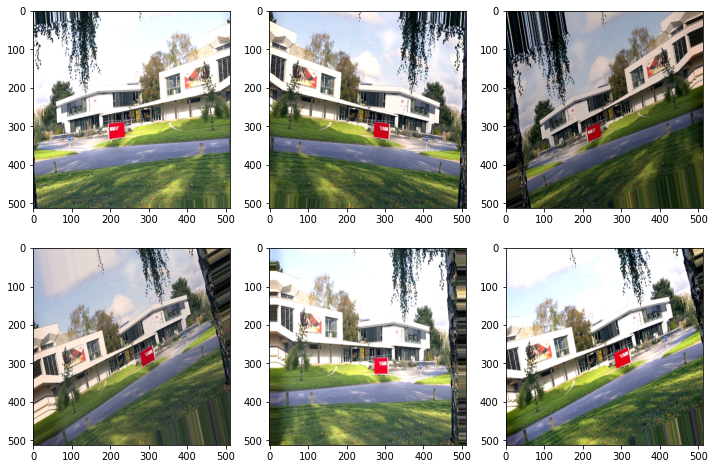
\includegraphics[width=12cm, height=6cm]{3-Figures/data_augmentation.png}}\\[0.5cm]
\caption{Data augmentation}
\label{fig:figure5}
\end{figure}

Comme le montre les images en dessus, à partir d'une image, nous avons pu générer cinq nouvelles images en utilisant la technique d'augmentation des données

\subsection{Les modèles de prédiction}
Parlons maintenant des modèles que nous avons formés sur notre dataset. On va évaluer les performances de chaque modele en calculant :  \textbf{\textcolor{blue}{Training accuracy}}et \textbf{\textcolor{blue}{Testing accuracy}}.

Training accuracy est la performance du modèle sur les images qu'il a apprises, Testing accuracy est la performance du modèle sur les images qu'il n'a jamais apprises.
\subsubsection{LBPH}
En raison de son pouvoir discriminant et sa   simplicité de calcul, le descripteur LBP est devenu une approche populaire dans diverses applications telles que la reconnaissance de visage par la suite on a décidé de l’utiliser en premier  pour effectuer la reconnaissance faciale.

\begin{figure}[H] 
\centering
\frame{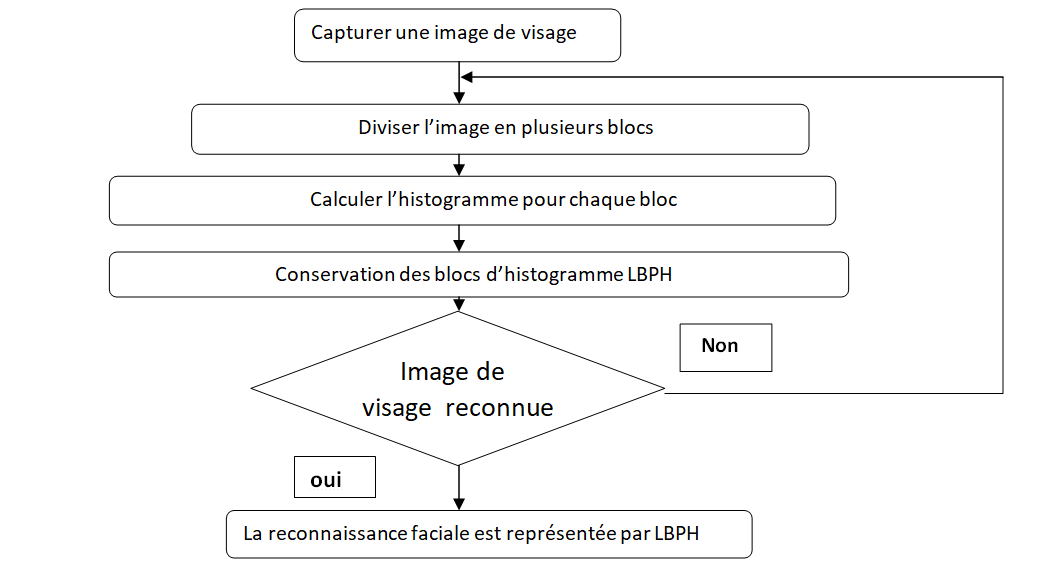
\includegraphics[width=12cm, height=6cm]{4-Images/lbph-archi.PNG}}\\[0.5cm]
\caption{LBPH}
\label{fig:figure5}
\end{figure}


Après avoir entraîné notre modèle LBPH sur la dataset de données, nous avons obtenu les résultats suivants:
\begin{figure}[H] 
\centering
\frame{\adjincludegraphics[width=11cm, height=1.7cm,clip]{4-Images/lbph-training.PNG}}\\[0.5cm]
\caption{LBPH-entraînement}
\label{fig:figure14}
\end{figure}

Nous pouvons voir que LBPH a classé toutes les images correctement, ce qui n'est pas un bon signe, car cela signifie qu'il a surajusté les données.
\begin{figure}[H] 
\centering
\frame{\adjincludegraphics[width=11cm, height=1.7cm,clip]{4-Images/lbph-testing.PNG}}\\[0.5cm]
\caption{LBPH-entraînement}
\label{fig:figure14}
\end{figure}
Si nous affichons la précision sur les images de test, nous voyons :

Le lien vers de Notebook d'entraînement de modèle : 
\href{https://github.com/mohammedAljadd/iEars/blob/main/Model%20training/Face%20identification/2-LBPH.ipynb}{LBPH}.

0.3 de précision est trop bas, LBPH ne pouvait pas classer les images qu'il n'a jamais apprises.

\subsubsection{CNN basique}
Un réseau neuronal convolutif (convolutional neural network - \textbf{CNN}) est un type de réseau neuronal artificiel utilisé dans la reconnaissance et le traitement d’images et spécifiquement conçu pour traiter les données de pixels.CNN est principalement utilisé dans les tâches d'analyse d'images telles que la \textbf{reconnaissance d'images}, la \textbf{détection d'objets} et la \textbf{segmentation}.
Le nom \textbf{convolutional neural network} vient de l'une des opérations les plus importantes du réseau : la convolution. \\

CNN se compose de plusieurs couches. La couche d'entrée qui est notre image, les couches cachées et la couche de sortie qui contient n unités où n est le nombre de classes que le modèle peut prédire.

\begin{figure}[H] 
\centering
\frame{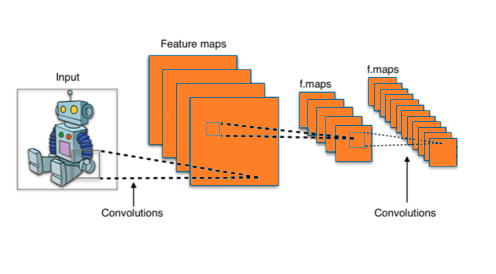
\includegraphics[width=12cm, height=6cm]{4-Images/cnn.png}}\\[0.5cm]
\caption{CNN}
\label{fig:figure6}
\end{figure}

En deep learning, une caractéristique (feature en anglais) est une propriété individuelle mesurable ou une caractéristique d'un phénomène. Le choix de caractéristiques informatives, discriminantes et indépendantes est un élément crucial des algorithmes efficaces de reconnaissance de formes, de classification et de régression. Ces caractéristiques aident le modèle à différencier les classes entre eux. Un exemple pourrait être la forme du corps d'un animal qui peut aider à identifier s'il s'agit d'un chien ou d'un chat. Plus nous avons de couches cachées, plus nous effectuons d'opérations de convolution, plus nous extrayons des caractéristique.

Après avoir entraîné notre modèle CNN sur dataset de données, nous avons obtenu les résultats suivants:
\begin{figure}[H] 
\centering
\frame{\adjincludegraphics[width=12cm, height=4cm,clip]{4-Images/cnn_training.PNG}}\\[0.5cm]
\caption{CNN-entraînement}
\label{fig:figure14}
\end{figure}


Une présision de 0.9595 montre que le modèle est bien entraîné.  Une précision de validation de 0.9480 montre que le modèle peut être généralisé à de nouvelles données et c'est le cas grâce à 0.94786232 dans l'image ci-dessous.

\begin{figure}[H] 
\centering
\frame{\adjincludegraphics[width=12cm, height=1.5cm,clip]{4-Images/cnn_test.PNG}}\\[0.5cm]
\caption{CNN-Test}
\label{fig:figure14}
\end{figure}

Le lien vers de Notebook d'entraînement de modèle : 
\href{https://github.com/mohammedAljadd/iEars/blob/main/Model%20training/Face%20identification/1-CNN%20model.ipynb}{CNN}


\subsubsection{VGG16}
Le VGG-16 est un réseau neuronal convolutif de 16 couches de profondeur. Une version pré-entraînée du réseau, entraînée sur plus d'un million d'images de la dataset ImageNet . Le réseau pré-entraîné peut classer les images dans 1000 catégories d'objets, telles que le clavier, la souris, le crayon et de nombreux animaux.\\[0.5cm]
\begin{figure}[H] 
\centering
\frame{\adjincludegraphics[width=12cm, height=8cm,clip]{4-Images/vgg16.PNG}}\\[0.5cm]
\caption{VGG16-1000classes}
\label{fig:figure14}
\end{figure}

Comme il n'est pas pratique d'entraîner un modèle VGG16 à partir de zéro, sinon cela prendrait des jours, nous avons entraîné un modèle pré-entraîné. Pour ce faire, nous avons supprimé la dernière couche, qui classait 1000 classes, et ajouté une couche de 5 classes pour notre projet :

\begin{figure}[H] 
\centering
\frame{\adjincludegraphics[width=15cm, height=3.5cm,clip]{4-Images/tune-vgg.PNG}}\\[0.5cm]
\caption{VGG16-5classes}
\label{fig:figure14}
\end{figure}

Avant de former le modèle, nous avons prétraité les données comme l'auteur de l'article de \href{https://arxiv.org/pdf/1409.1556.pdf}{VGG16} cité comme mentionné dans l'image suivante :

\begin{figure}[H] 
\centering
\frame{\adjincludegraphics[width=10cm, height=3cm,clip]{4-Images/vgg16.preprocessing.jpg}}\\[0.5cm]
\caption{VGG16-prétraitement}
\label{fig:figure19}
\end{figure}
Donc, Le seul prétraitement effectué est la soustraction de la valeur RGB moyenne. Nous montrons dans l'image suivante un exemple du prétraitement qui est effectué avant d'utiliser les données pour l'entraînement du modèle:
\begin{figure}[H] 
\centering
\frame{\adjincludegraphics[width=10cm, height=6cm,clip]{3-Figures/preprocess_vgg_example.PNG}}\\[0.5cm]
\caption{VGG16-prétraitement-exemple}
\label{fig:figure19}
\end{figure}


Après avoir entraîné notre modèle VGG16 sur dataset de données, nous avons obtenu les résultats suivants:
\begin{figure}[H] 
\centering
\frame{\adjincludegraphics[width=15cm, height=4cm,clip]{4-Images/vgg-training.jpg}}\\[0.5cm]
\caption{VGG-entraînement}
\label{fig:figure14}
\end{figure}


Une précision de 0.991 montre que le modèle est bien entraîné.  Une précision de validation de 0.9857 montre que le modèle peut être généralisé à de nouvelles données et c'est le cas grâce à 0.9882 dans l'image ci-dessous.

\begin{figure}[H] 
\centering
\frame{\adjincludegraphics[width=8cm, height=1.5cm,clip]{4-Images/vgg-testing.jpg}}\\[0.5cm]
\caption{VGG-Test}
\label{fig:figure14}
\end{figure}


Le lien vers de Notebook d'entraînement de modèle : 
\href{https://github.com/mohammedAljadd/iEars/blob/main/Model%20training/Face%20identification/3-VGG%2016.ipynb}{VGG16}


\subsubsection{FaceNet}
FaceNet est un réseau neuronal profond utilisé pour extraire les caractéristiques d'une image du visage d'une personne. Il a été publié en 2015 par les chercheurs de Google Schroff. Son mode de fonctionnement est simple il prend une image du visage de la personne en entrée et produit un vecteur de 128 nombres qui représentent les caractéristiques les plus importantes d'un visage. En apprentissage automatique, ce vecteur est appelé Embedding layer et toutes les informations importantes de l'image sont intégrées dans ce vecteur. 
\begin{figure}[H] 
\centering
\frame{\adjincludegraphics[width=7cm, height=5cm,clip]{4-Images/facenet_archi.PNG}}\\[0.5cm]
\caption{FaceNet}
\label{fig:figure14}
\end{figure}

Idéalement, embedding layers de visages similaires sont également similaires.

On pourra facilement l'extraire en python:
\begin{figure}[H] 
\centering
\frame{\adjincludegraphics[width=8cm, height=5cm,clip]{4-Images/embedding_layer.PNG}}\\[0.5cm]
\caption{Embedding layer}
\label{fig:figure14}
\end{figure}

FaceNet a obtenu une précision de près de 100 \% sur une dataset de données de reconnaissance faciale populaire appelé Labeled Faces in the Wild, qui comprend plus de 13 000 photos de visages provenant de l'ensemble du Web.



Le lien vers de Notebook d'entraînement de modèle : 
\href{https://github.com/mohammedAljadd/iEars/blob/main/Model%20training/Face%20identification/4-FaceNet.ipynb}{FaceNet}


\subsection{Comparison}
\subsection{Haar cascade classifier}
La détection d'objets à l'aide de classificateurs en cascade basés sur les caractéristiques Haar est une méthode efficace de détection d'objets proposée par Paul Viola et Michael Jones dans leur article "Rapid Object Detection using a Boosted Cascade of Simple Features" en 2001. Il s'agit d'une approche basée sur l'apprentissage automatique dans laquelle une fonction en cascade est entraînée à partir d'un grand nombre d'images positives et négatives. Elle est ensuite utilisée pour détecter des objets dans d'autres images.
On va utiliser ce classificateur pour détecter les visages des personnes dans une image
\label{sec:haar}

\section{Prédiction de texte}
\subsection{Tesseract OCR}
Tesseract est un logiciel de reconnaissance optique de caractères sous licence Apache.

Conçu par les ingénieurs de Hewlett Packard de 1985 à 1995, son développement est abandonné pendant les dix années suivantes ; en 2005, les sources du logiciel sont publiées sous licence Apache et Google poursuit son développement. Initialement limité aux caractères ASCII, il reconnaît les caractères UTF-8 dans plus de 100 langues.\\[0.5cm]

\begin{figure}[H] 
\centering
\frame{\adjincludegraphics[width=10cm, height=5cm,clip]{4-Images/ocr.PNG}}\\[0.5cm]
\caption{Tesseract OCR}
\label{fig:figure14}
\end{figure}

\subsection{HTR}
La reconnaissance de l’écriture manuscrite (en anglais, handwritten text recognition ou HTR) est un traitement informatique qui a pour but de traduire un texte écrit en un texte codé numériquement.

Notre modèle HTR fonctionne sur des images qui ne contiennent qu'une seule ligne, nous devons donc effectuer un prétraitement que nous expliquerons dans la section suivante. 
\subsubsection{Ségmentation}
Comme le modèle de reconnaissance de texte ne fonctionne que sur des caractères uniques, l'image ne contient qu'un seul caractère, nous devons segmenter l'image en caractères avant de la soumettre à notre modèle.
Il existe trois niveaux de segmentation : 
\begin{itemize}
    \item Segmentation au niveau des lignes.
    \item Segmentation au niveau des mots.
    \item Segmentation au niveau des caractères.
\end{itemize}

On prend une image pour faire la segmentation :
\begin{figure}[H] 
\centering
\frame{\adjincludegraphics[width=8cm, height=5cm,clip]{4-Images/htr-test.PNG}}\\[0.5cm]
\end{figure}
Nous allons d'abord faire un prétraitement. Aprés, Nous utiliserons la méthode du histogramme pour segmenter l'image.

\subsubsection*{Segmentation au niveau des lignes :}
Grâce à cette méthode, nous pouvons savoir où se trouvent les lignes dans l'image:



\begin{figure}[H]
    \centering
    \subfloat{{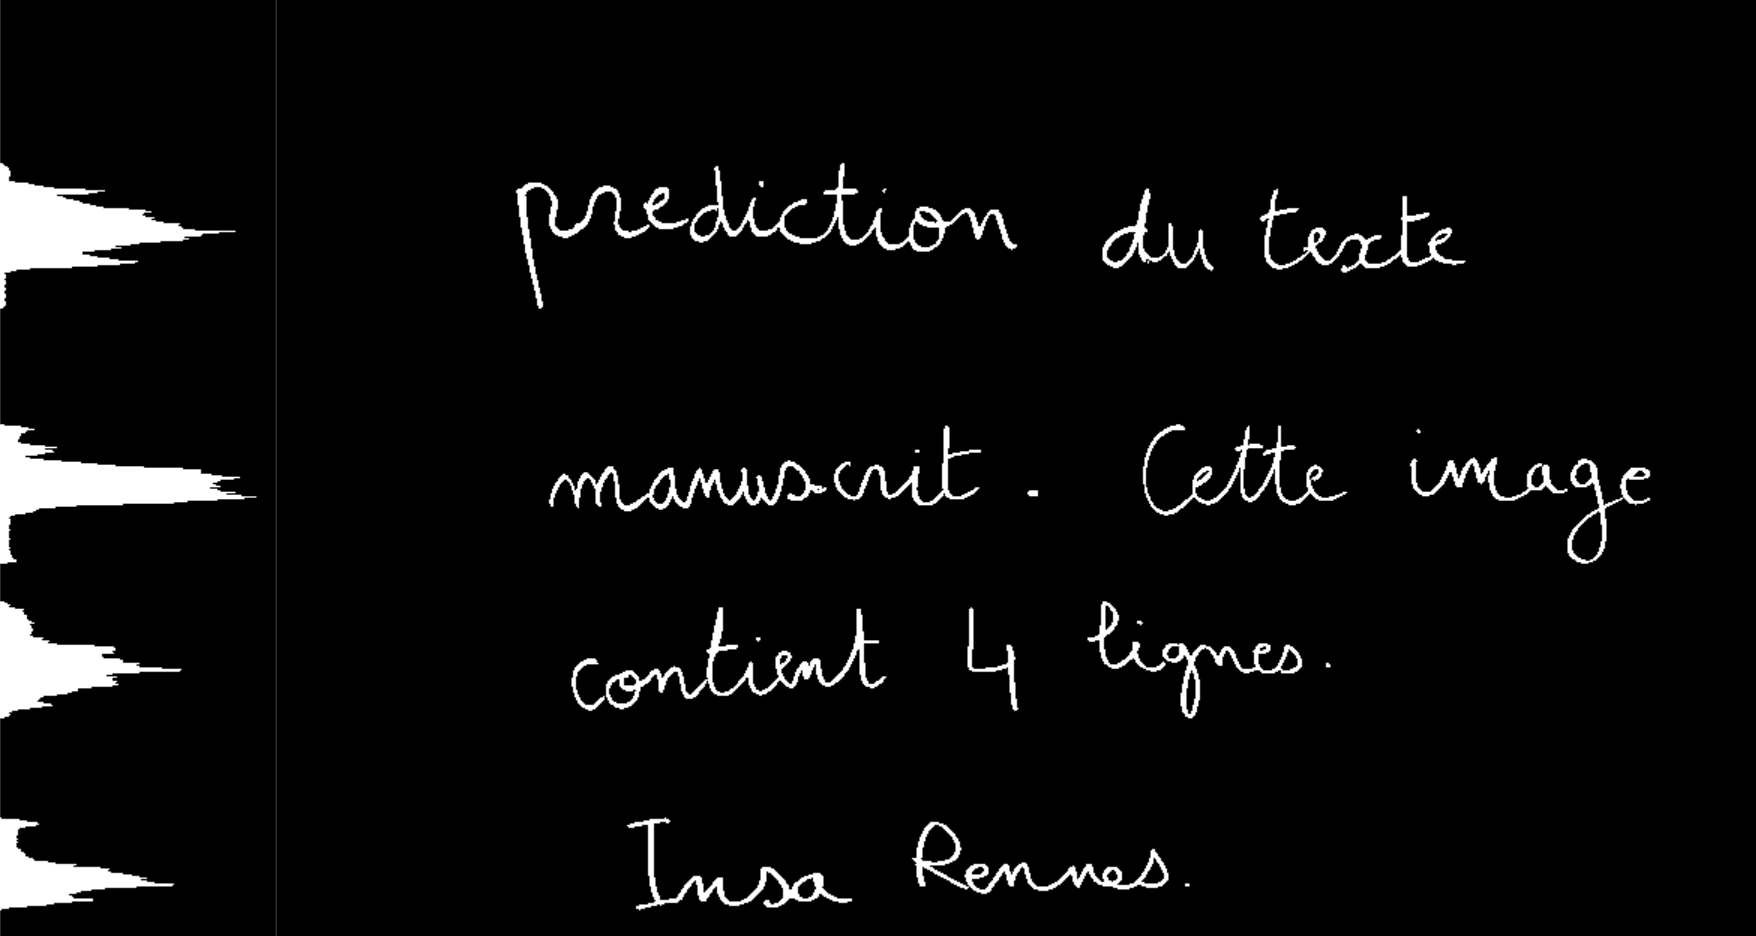
\includegraphics[width=5cm]{4-Images/level1-segmentation.PNG} }}
    \qquad
    \subfloat{{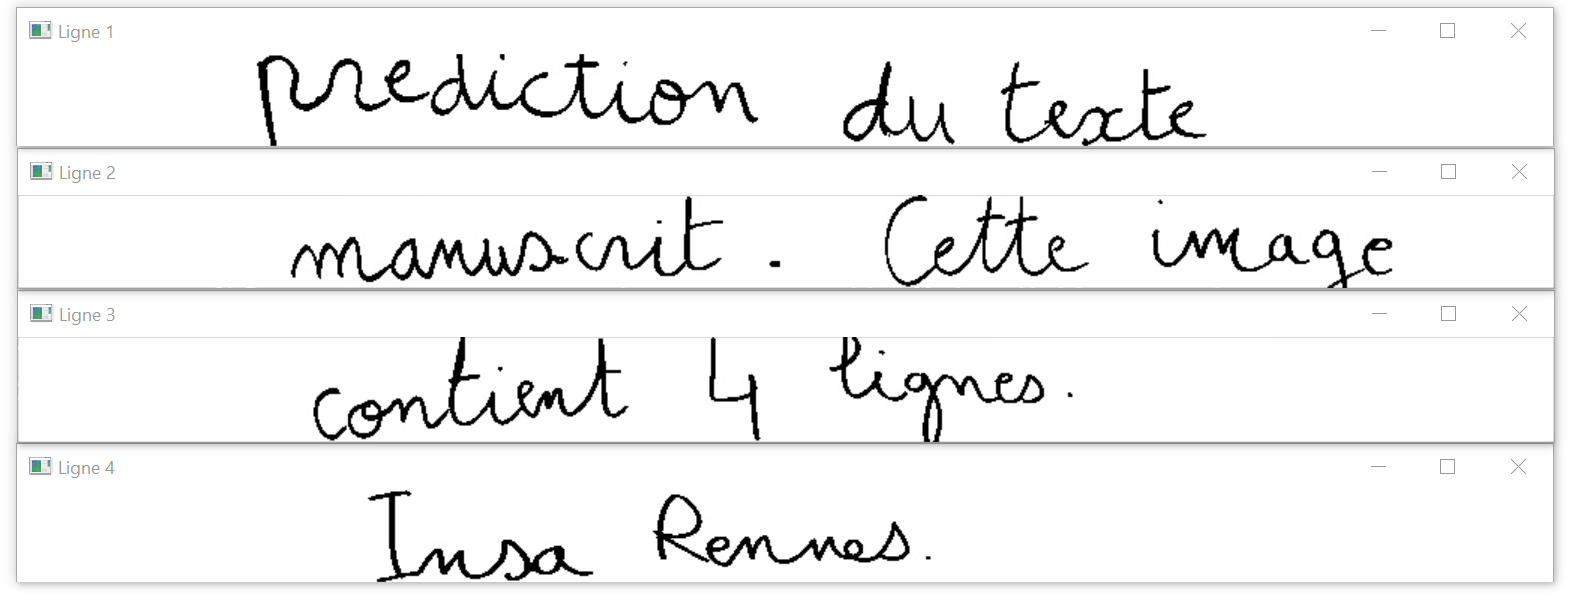
\includegraphics[width=5cm]{4-Images/level1-lines.PNG} }}
    \caption{Segmentation au niveau1}
    \label{fig:example}
\end{figure}


\subsubsection*{Segmentation au niveau des mots :}
Nous pouvons aussi détecter les mots de chaque ligne comme le montre l'image suivante :

\begin{figure}[H] 
\centering
\frame{\adjincludegraphics[width=8cm, height=5cm,clip]{4-Images/level2-words.PNG}}\\[0.5cm]
\caption{Segmentation au niveau2}
\label{fig:figure20}
\end{figure}

\subsubsection*{Segmentation au niveau des lettres :}
La troisième étape consiste à détecter les lettres de chaque mot:

\section{Prédiction d'objets}
YOLO (You Only Look Once) est un algorithme de détection et de reconnaissance d'objets qui est trés puissant en terme de traitement en temps réel.

Notion d’ancre : En réalisant une analyse préalable sur les délimitations des objets que l’on essaie de trouver, Notre système modélise la détection comme un problème de régression. Il divise l'image en une grille régulière et prédit simultanément les boîtes de délimitation, la confiance dans ces boîtes,et les probabilités de classe. Ces prédictions sont encodées sous la forme d'un tenseur : 
\begin{center}
    S × S × (B × 5 + C).\\
    C : nombre de classe
\end{center}



\begin{figure}[H] 
\centering
\frame{\adjincludegraphics[width=10cm, height=5cm,clip]{4-Images/yolo-principe.PNG}}\\[0.5cm]
\caption{Principe de YOLO}
\label{fig:figure18}
\end{figure}


Fonction d’activation : Nous utilisons une fonction d'activation linéaire pour la couche finale et toutes les autres couches utilisent l'activation linéaire rectifiée par fuite (\textbf{Leaky-relu}) suivante :\\
\begin{center}
    $\phi$(x) = x, si $x > 0$ \\
    0.1x, Sinon
\end{center}
 

\begin{figure}[H] 
\centering
\frame{\adjincludegraphics[width=10cm, height=5cm,clip]{4-Images/leaky-relu.PNG}}\\[0.5cm]
\caption{Fonction d'activations}
\label{fig:figure18}
\end{figure}


Trouver les ancres : L’IoU – ou Intersection over Union – est une façon de mesurer la qualité de la détection d’un objet en comparant, dans un dataset d’entraînement, la position connue de l’objet dans l’image avec la prédiction faite par l’algorithme. L’IoU est le rapport entre la surface de l’intersection des bounding box considérées et la surface de l’union des ensembles.
\begin{figure}[H] 
\centering
\frame{\adjincludegraphics[width=9cm, height=5cm,clip]{4-Images/iou.PNG}}\\[0.5cm]
\caption{IoU}
\label{fig:figure18}
\end{figure}


\subsection{Dataset}
Pour créer un détecteur d'objets personnalisé, On a  besoin d'un bon ensemble de données d'images et d'étiquettes afin que le détecteur puisse être entraîné efficacement à détecter des objets. On utilise alors Open images dataset v6.
Ensuite une chose essentielle a traiter  est les annotations.

Annotation :
Dans la dataset originale, les coordonnées des boîtes de délimitation sont établies de la manière suivante :

XMin, XMax, YMin, YMax : coordonnées de la boîte, en coordonnées d'image normalisées. XMin est dans [0,1], où 0 est le pixel le plus à gauche, et 1 est le pixel le plus à droite dans l'image. Les coordonnées Y vont du pixel supérieur (0) au pixel inférieur (1).

Cependant, afin de permettre une représentation plus intuitive et de donner un maximum de flexibilité, chaque annotation .txt est faite comme suit :
\begin{center}
    $name\_of\_the\_class left top right bottom$
\end{center}
\begin{figure}[H] 
\centering
\frame{\adjincludegraphics[width=7cm, height=5cm,clip]{4-Images/annotation.PNG}}\\[0.5cm]
\caption{Annotation YOLOv4}
\label{fig:figure18}
\end{figure}

Étapes pratiques :

Au début on télécharge notre base de données d’images pour entrainer notre modèle ( dataset ) . Ceci en passant par les étapes que je résume ci-dessous :


\begin{itemize}
    \item \textbf{git clone https://github.com/theAIGuysCode/OIDv4$\_$ToolKit.git} \\
Il s’agit ici de télécharger le logiciel qui permet de récupérer la dataset a partir de open images dataset v6.
    \item \textbf{cd $C:\backslash classe\backslash OIDv4\_$ToolKit}\\
    On accède au dossier ou on doit télécharger la dataset 
    \item \textbf{pip install -r requirements.txt}
On installe des éléments python nécessaire pour le traitement de la dataset. 
    \item \textbf{python main.py downloader --classes (Nom des classes qu'on veut) --type csv train --limit 800 --multiclasses 1}
    \item On modifie les noms des classes dans le fichier classes.txt.
    \item Pour former les annotations on exécute un code python comme suit  : python convert$\_$annotations.py.
    
\end{itemize}


\begin{figure}[H] 
\centering
\frame{\adjincludegraphics[width=10cm, height=5cm,clip]{4-Images/dataset-yolo.PNG}}\\[0.5cm]
\caption{Dataset détection d'objet}
\label{fig:figure14}
\end{figure}

YOLO v4 a déjà été entraîné sur un jeu de données coco qui contient 80 classes qu'il peut prédire. Nous allons récupérer ces poids pré-entraînés afin de pouvoir exécuter YOLO v4 sur d’autres classes et obtenir des détections personnalisées.

\begin{figure}[H] 
\centering
\frame{\adjincludegraphics[width=8cm, height=5cm,clip]{4-Images/reseaux.PNG}}\\[0.5cm]
\caption{Réseau YOLO}
\label{fig:figure14}
\end{figure}




\subsection{YOLOv4 entraînement}
Maintenant qu’on a préparé les outils nécessaires pour notre détection , on va lancé la phase d'entraînement sur Google colab ( environnement de développement qui nous propose des ressources matérielles importantes dans le cloud ) vu la grande masse de données qu'on essaie de manipuler.
A l’issue de cette dernière étape on obtiendrait un fichier  .weights regroupant les nouveau paramètre du modèle .

\begin{figure}[H] 
\centering
\frame{\adjincludegraphics[width=8cm, height=3cm,clip]{4-Images/Google-Colab.PNG}}\\[0.5cm]
\caption{Google Colab}
\label{fig:figure17}
\end{figure}

\subsection{YOLOv4 3-classes}
Après l'entraînement du modèle, nous avons obtenu les résultats suivants :  

\begin{figure}[H]
    \centering
    \subfloat[Person]{{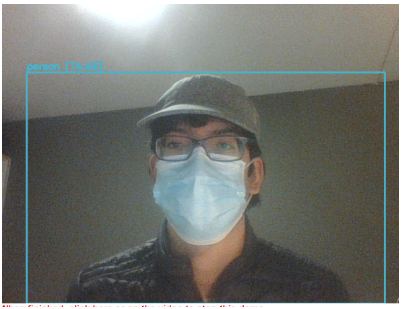
\includegraphics[width=4cm]{4-Images/ahmed.PNG} }}
    \qquad
    \subfloat[Laptop]{{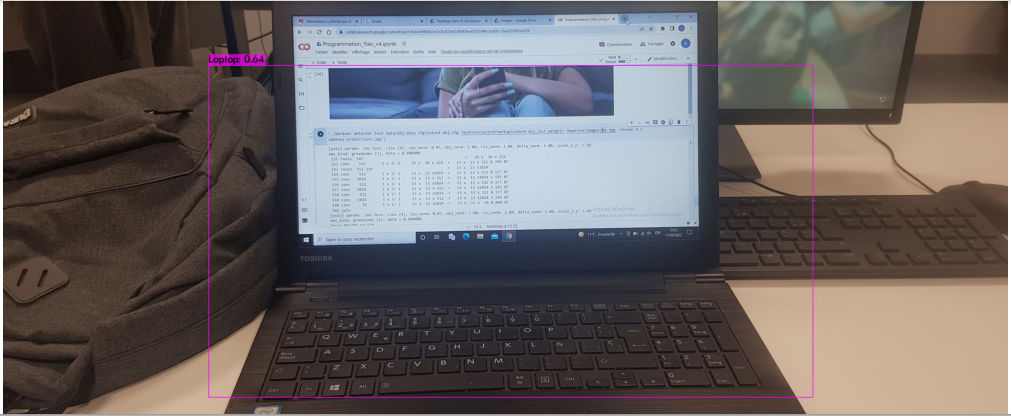
\includegraphics[width=5cm]{4-Images/laptop.PNG} }}
    \qquad
    \subfloat[Laptop]{{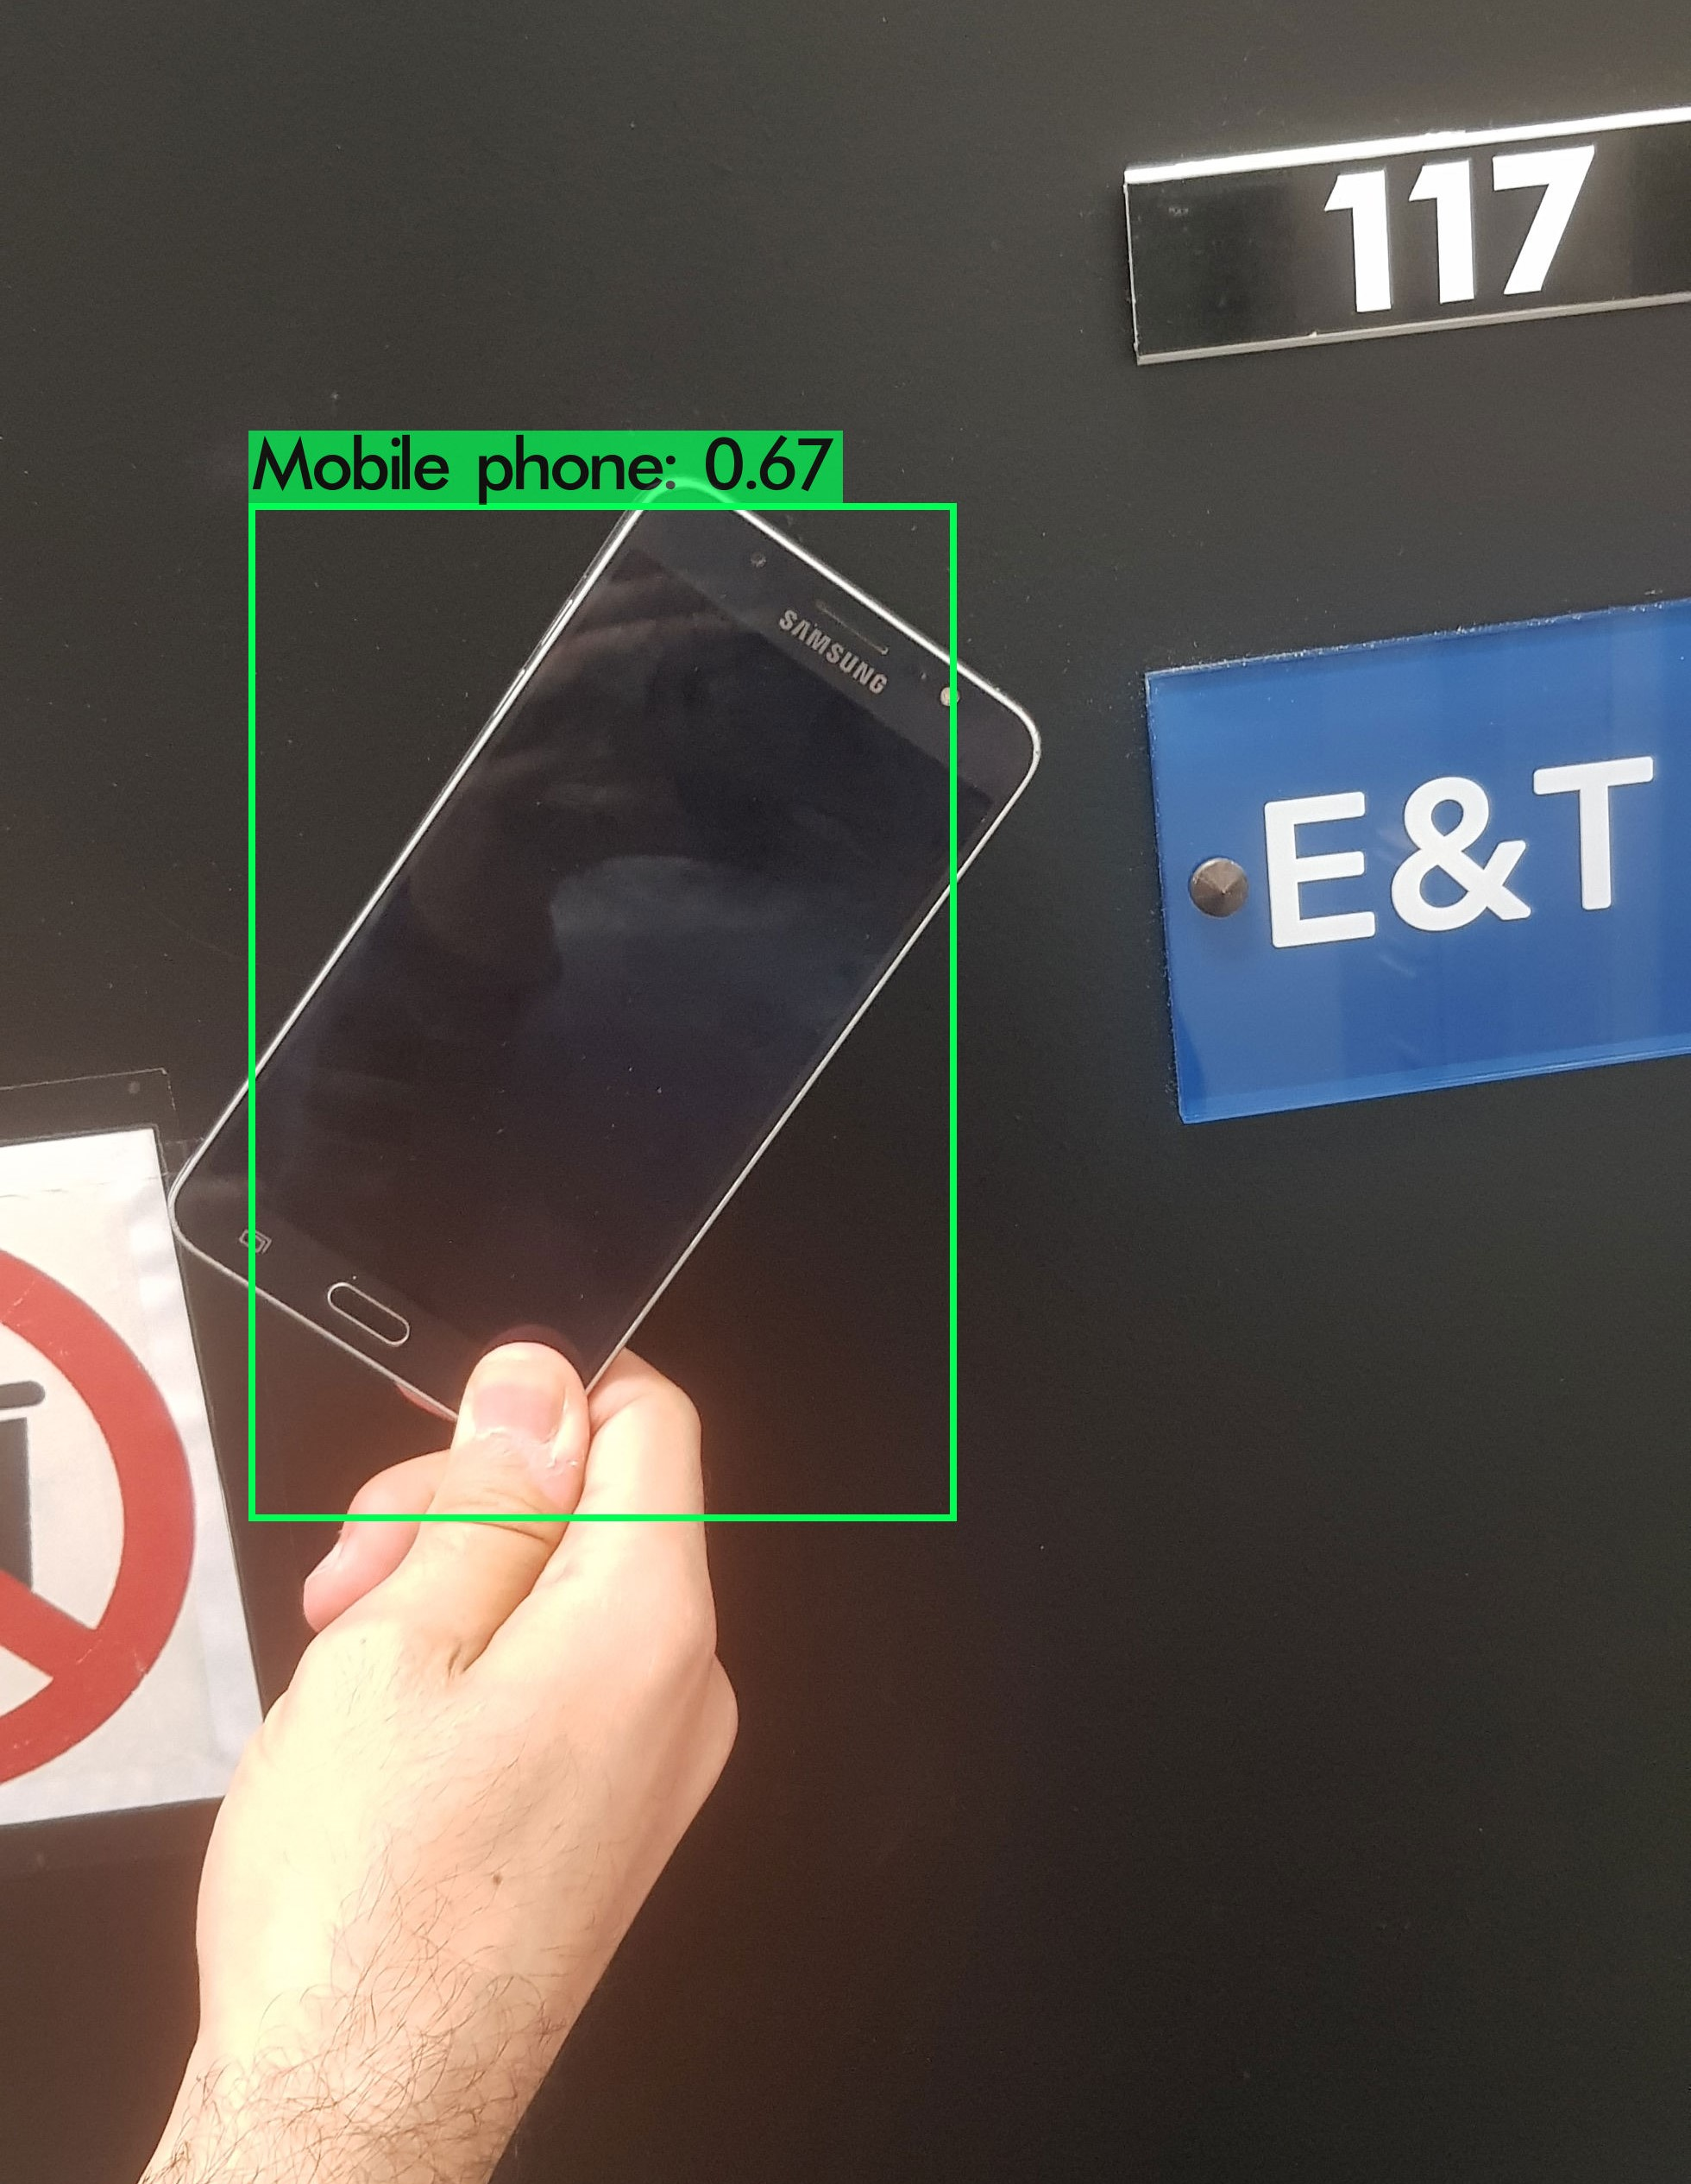
\includegraphics[width=2.5cm, height=3.3cm]{4-Images/detection-mobile.jpg} }}
    \caption{Résultats YOLO-3 classes}
    \label{fig:example}
\end{figure}

\subsection{YOLOv4 8-classes}
On va suivre les mêmes étapes pour le modèle précédent de 3 classes or la masse de données à utiliser devient plus importantes et la phase d'entraînement peut engendrer des erreurs et par conséquent ne pas bien détecter une classe .
Solution : On a pensé alors à diviser l'entraînement en des sous-classes et les exécuter après séquentiellement .

\begin{figure}[H] 
\centering
\frame{\adjincludegraphics[width=11cm, height=2.8cm,clip]{4-Images/classe8.PNG}}\\[0.5cm]
\caption{Les 8 classes YOLOv4}
\label{fig:figure17}
\end{figure}

\begin{figure}[H]
    \centering
    \subfloat[Whiteboard]{{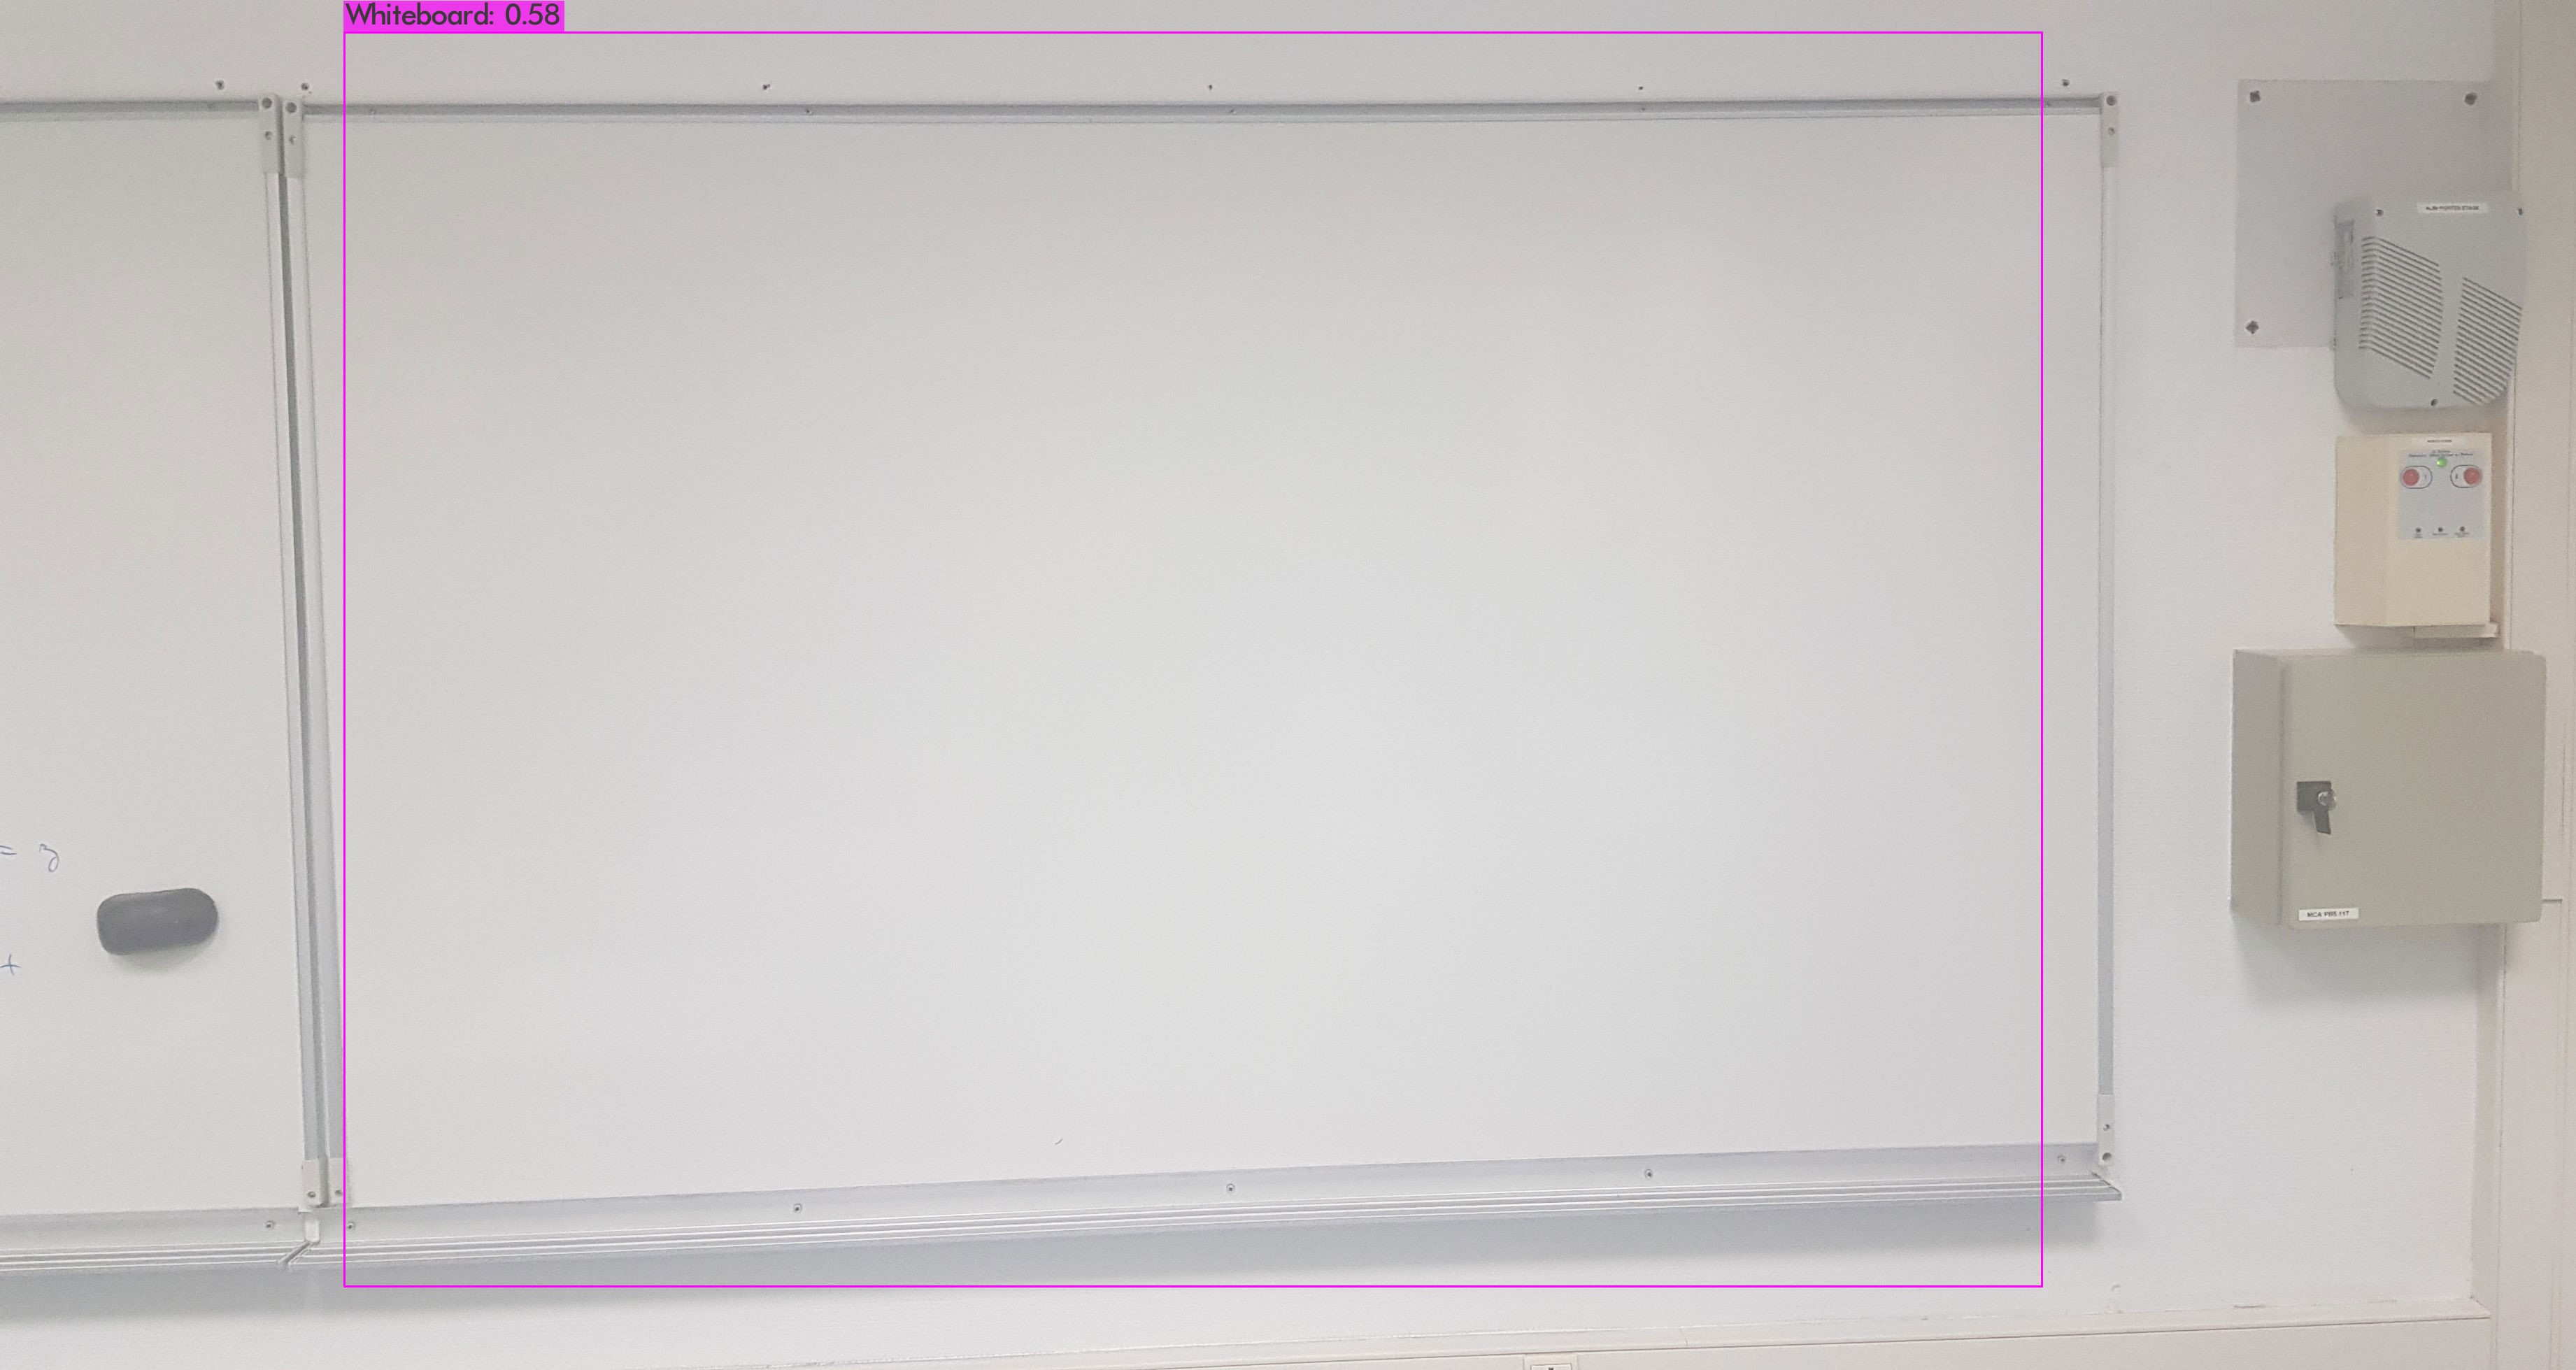
\includegraphics[width=7cm, height=4cm]{4-Images/whiteboard.jpg} }}
    \qquad
    \subfloat[Computer mouse]{{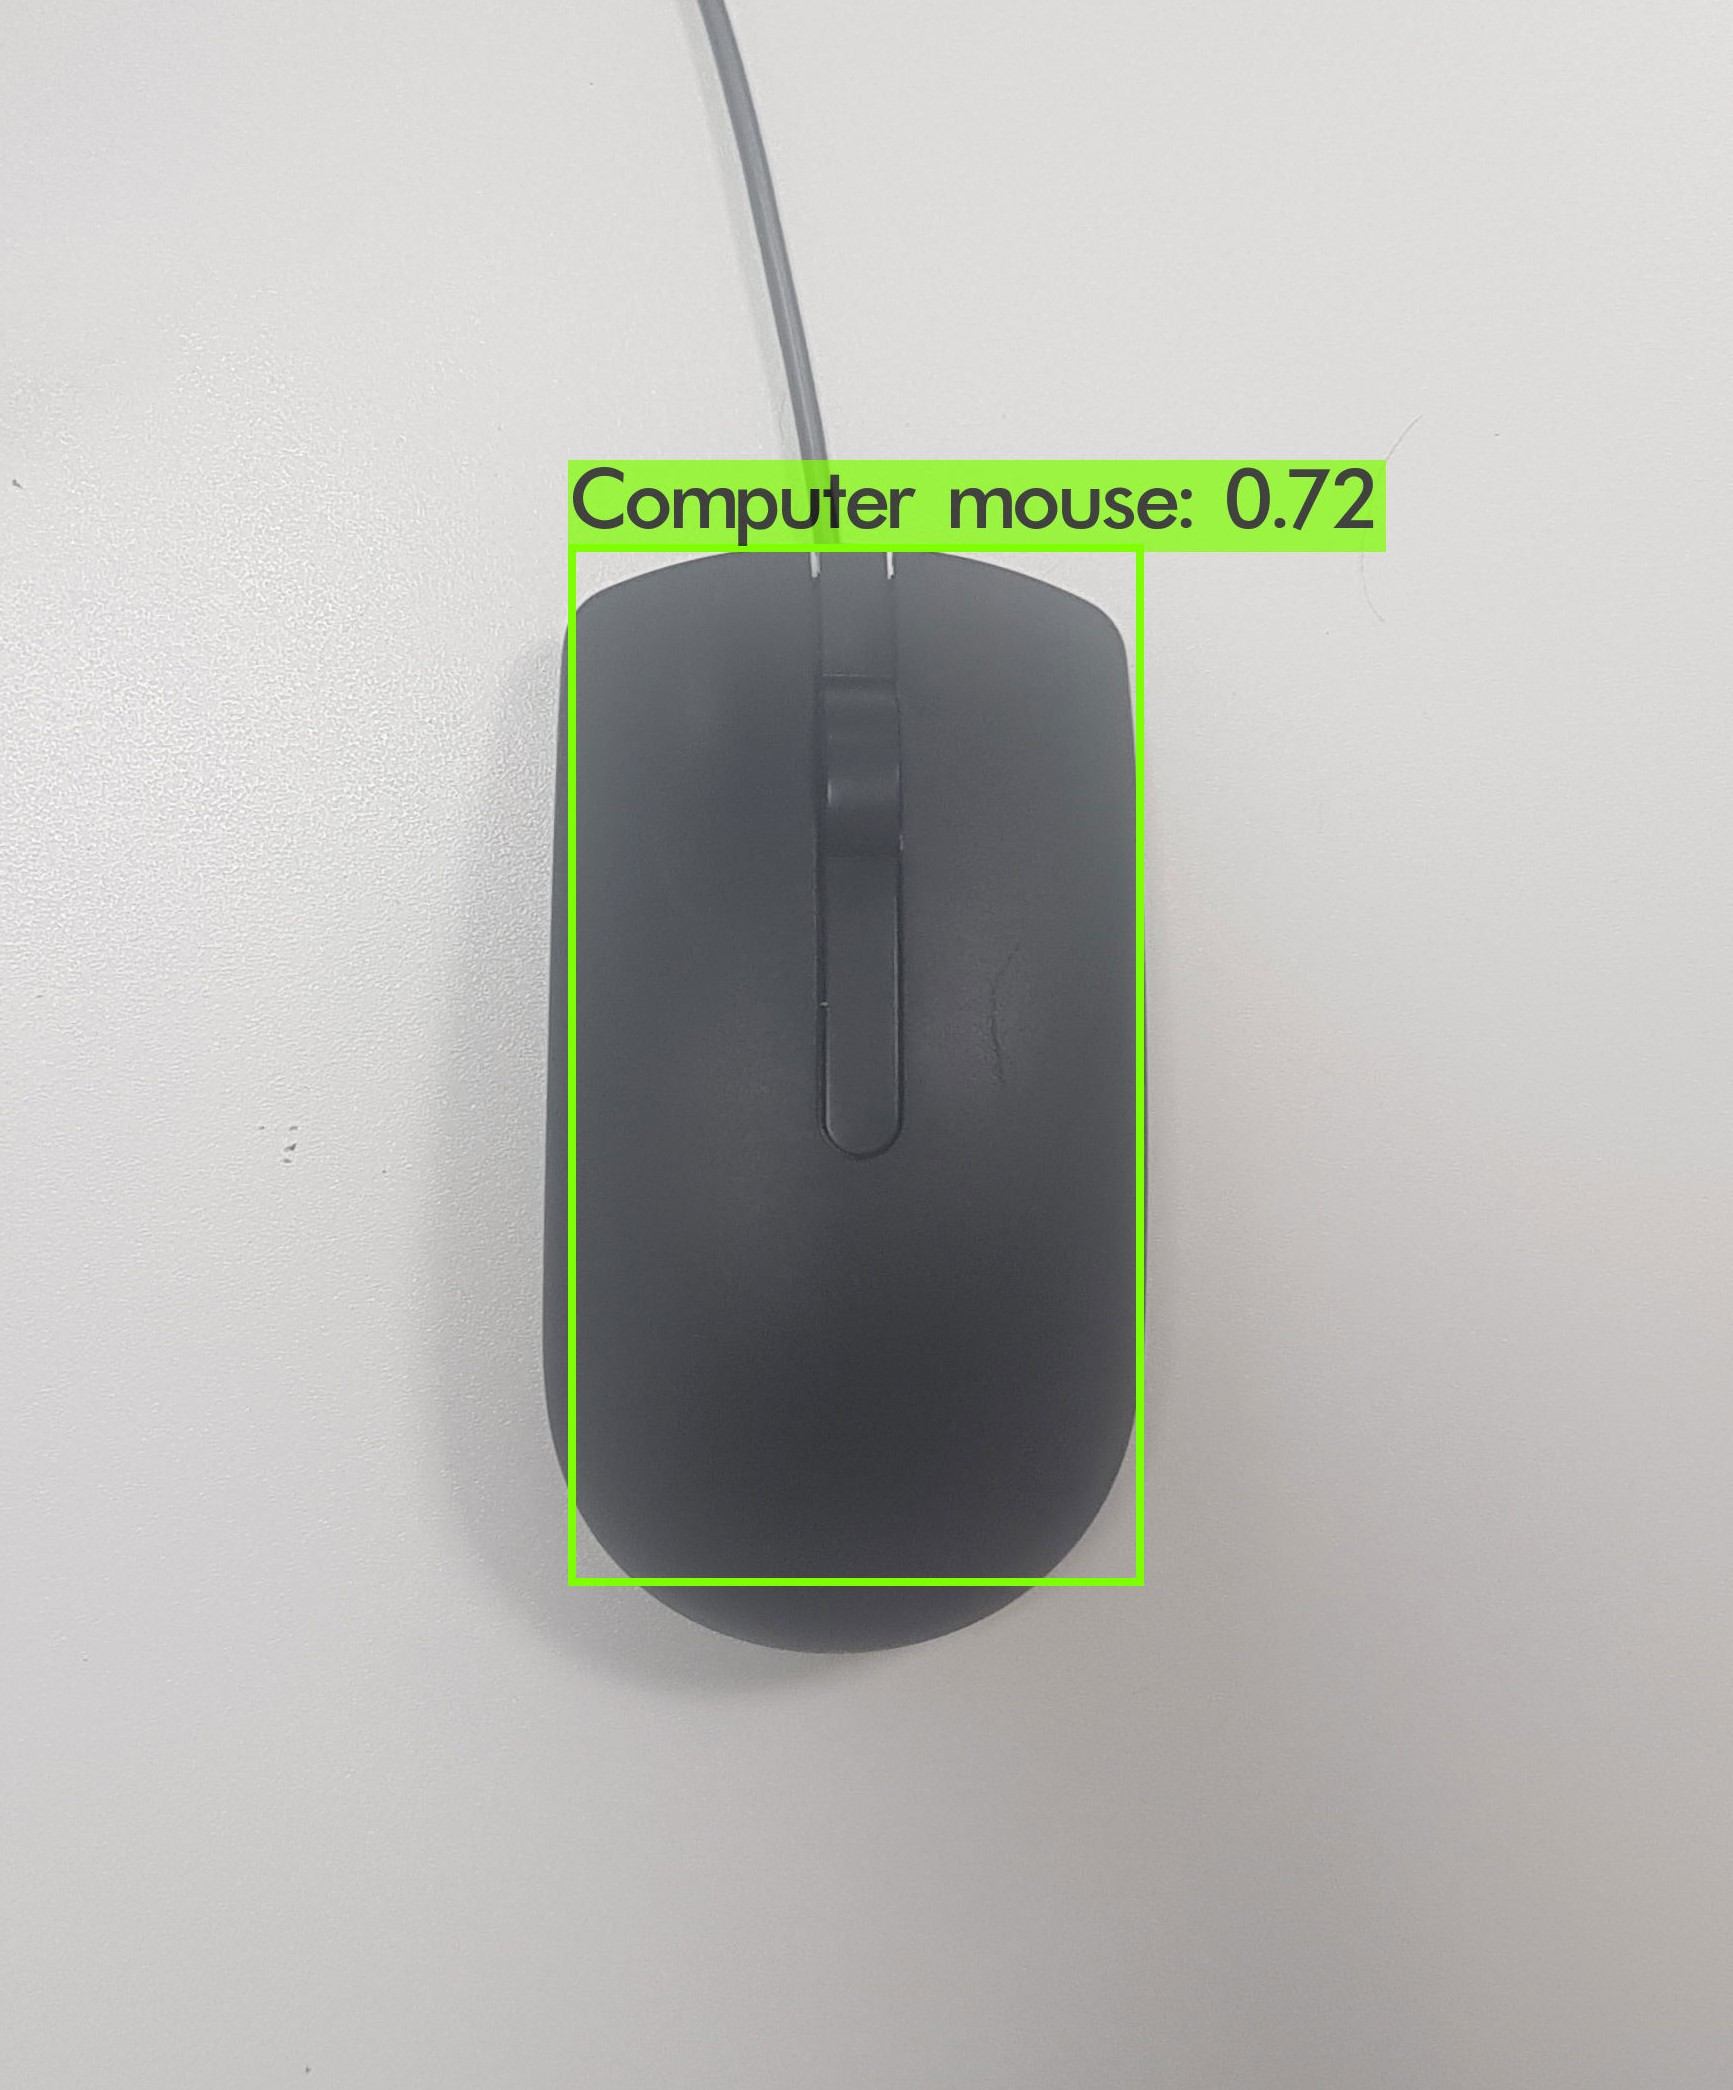
\includegraphics[width=3cm, height=4cm]{4-Images/mouse.jpg} }}
    \qquad
    \subfloat[Bottle]{{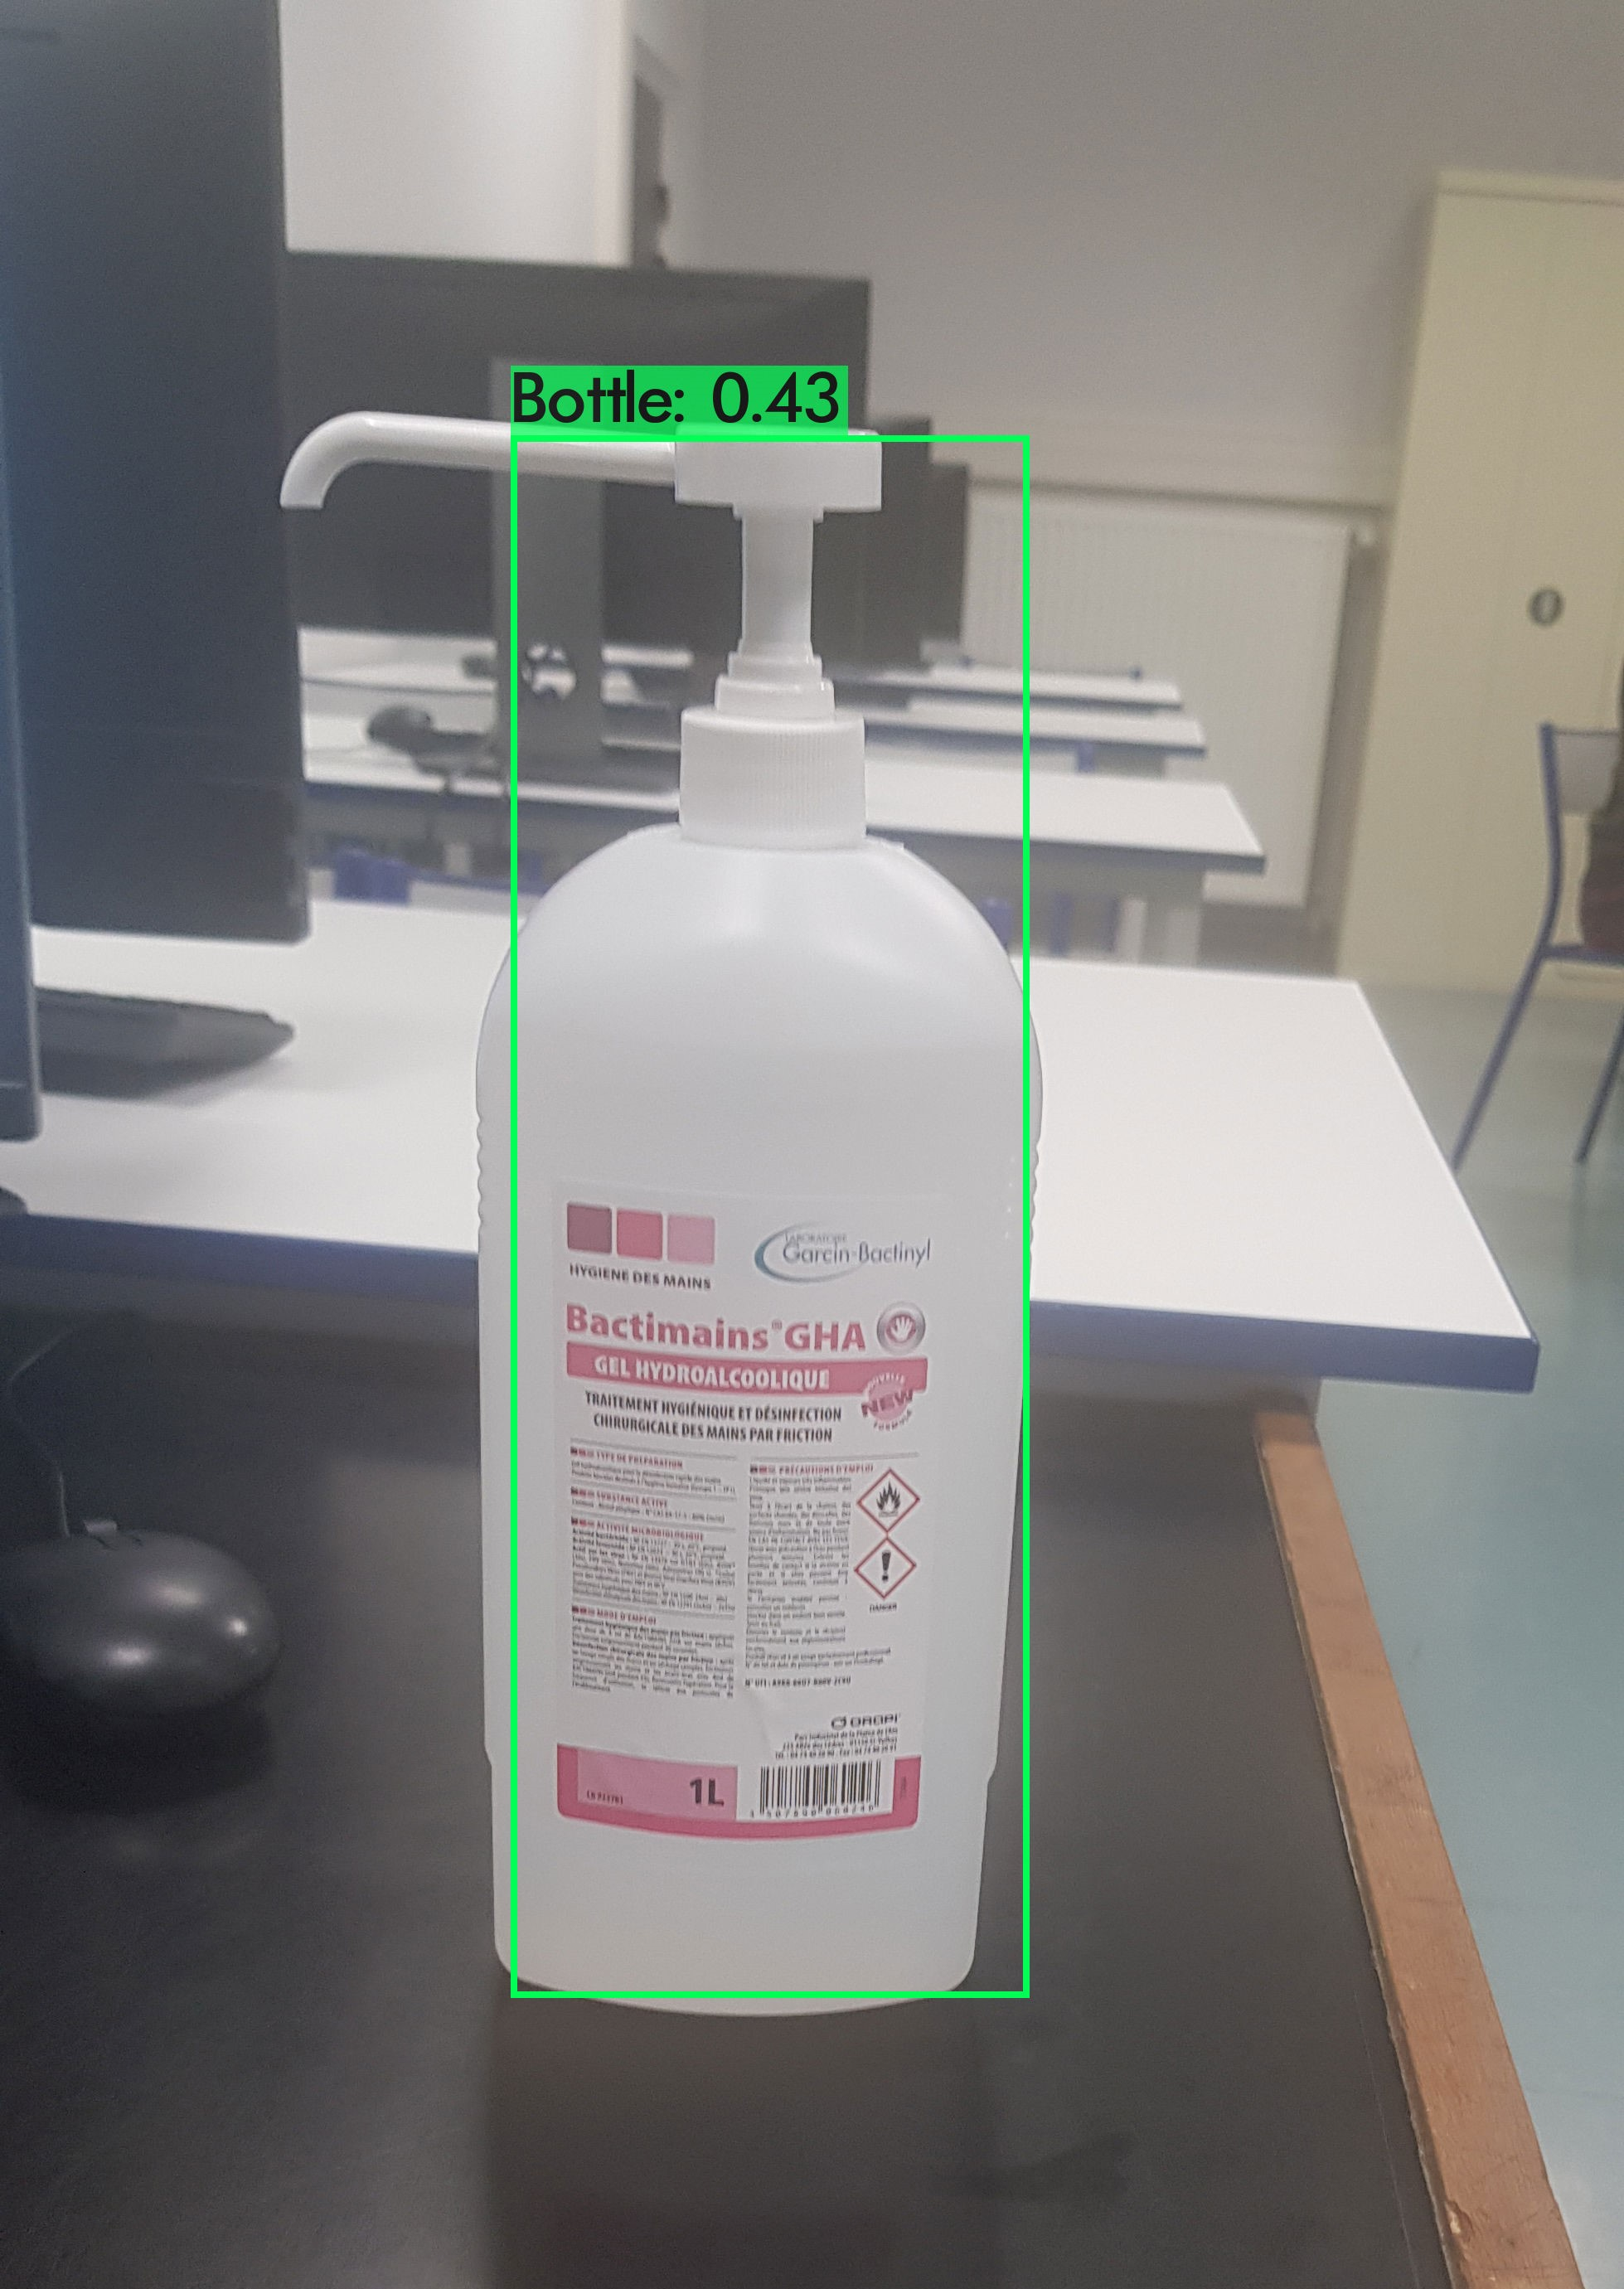
\includegraphics[width=3cm, height=4cm]{4-Images/bottle.jpg} }}
    \caption{Résultats YOLO-8 classes}
    \label{fig:example}
\end{figure}

\subsection{YOLOv4 80-classes}
L'algorithme que nous utiliserons à la fin peut détecter 80 classes. La liste des 80 objects est présentée dans ce lien : \href{https://github.com/mohammedAljadd/iEars/blob/main/coco-dataset-list/coco.names}{Coco-dataset}.

% Chapter 4 Version I ---------------------------------------------------------
% -------------------------------------------------------------------

\pagebreak
\lhead{Serveur}

\chapter{Serveur}\thispagestyle{fancy}

\section{Mode I : Traitement image}\thispagestyle{fancy}
\subsection{Schéma}
\subsection{API}
En informatique, une \textbf{API} (application programming interface) ou interface de programmation applicative est un ensemble normalisé de classes, de méthodes, de fonctions et de constantes qui sert de façade par laquelle un logiciel offre des services à d'autres logiciels. Elle est offerte par une bibliothèque logicielle ou un service web, le plus souvent accompagnée d'une description qui spécifie comment des programmes consommateurs peuvent se servir des fonctionnalités du programme fournisseur.\\[0.5cm]

De manière plus générale, on parle d'\textbf{API} à partir du moment où une entité informatique cherche à agir avec ou sur un système tiers, et que cette interaction se fait de manière normalisée en respectant les contraintes d'accès définies par le système tiers. On dit que le système tiers « expose une \textbf{API}». À ce titre, des choses aussi diverses que la signature d'une fonction, une \textbf{URL} … sont parfois considérés comme des API (ou \textbf{micro-API}) à part entière.\\[0.5cm]

% include {float} package and add [h] to prevent putting the figure in the end of the chapter
\begin{figure}[H] 
\centering
\frame{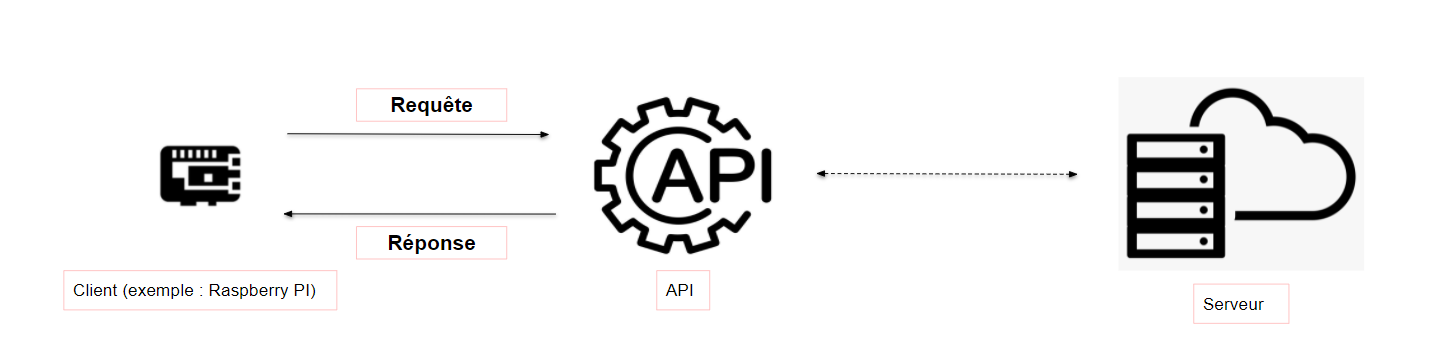
\includegraphics[width=17cm, height=5cm]{3-Figures/client-server-archi.PNG}}\\[0.5cm]
\caption{API}
\label{fig:figure7}
\end{figure}

L'image ci-dessus montre l'architecture client-serveur où l'on voit clairement l'API entre le serveur et le client. Le client envoie une requête à l'API pour demander des services au serveur, ce dernier transmettra la requête au serveur afin qu'il renvoie la réponse au client.

Il y a un type d'API qui s'appele \textbf{REST API} (\textbf{Representational State Transfer Application Program Interface}) est un style architectural qui permet aux logiciels de communiquer entre eux sur un réseau ou sur un même appareil. Le plus souvent les développeurs utilisent des API REST pour créer des services web. Souvent appelés services web RESTful, REST utilise des méthodes HTTP pour récupérer et publier des données entre un périphérique client et un serveur.

Le concept fondamental de toute \textbf{REST API} est la ressource. Une ressource est un objet avec un type, des données associées, des relations avec d'autres ressources et un ensemble de méthodes qui fonctionnent dessus.

En rapport avec notre project, les ressources qu'on possède sont les trois services suivantes : Prédiction visage, prédiction de texte et prédiction d'objets.\\[0.5cm]

\begin{figure}[H] 
\centering
\frame{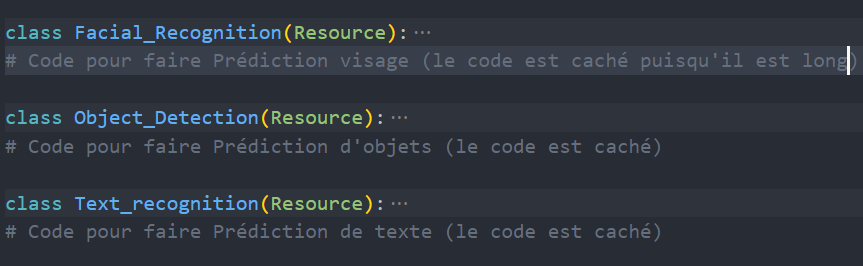
\includegraphics[width=17cm, height=5cm]{3-Figures/resources.PNG}}
\caption{Ressources d'API}
\label{fig:figure8}
\end{figure}
Chaque ressource est définie par une URL dont la première partie est l'adresse IP du serveur et la deuxième est un chemin spécifique qui commence par "/" comme le montre l'image en dessous.

\begin{figure}[H] 
\centering
\frame{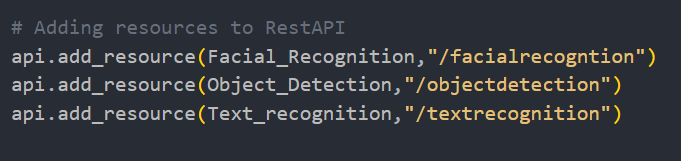
\includegraphics[width=13cm, height=3cm]{3-Figures/add-resources.PNG}}
\caption{Ajout des ressources}
\label{fig:figure9}
\end{figure}

Donc on a ajouté les ressources à notre variable \textbf{api} en spécifiant les chemins pour distinguer entre les 3 ressources. Si par exemple le client veut bénéficier du premier service et que le serveur a l'adresse ip suivante \textbf{\textcolor{blue}{10.1.1.18}}, le client enverra une requête HTTP à \textbf{\textcolor{blue}{'http://10.1.1.18/facialrecognition'}} contenant une image et il recevra en retour le résultat de la prédiction. Tout cela est du côté serveur, nous montrerons ensuite ce qui se passe du côté client

    \subsection{Test avec Postman}

Postman est une application utilisée pour les tests d'API. Il s'agit d'un client HTTP qui teste les requêtes HTTP, en utilisant une interface utilisateur graphique, à travers laquelle nous obtenons différents types de réponses qui doivent ensuite être validées. On spécifie le chemin pour envoyer la requête HTTP et on choisit une image à envoyer.

\begin{figure}[H] 
\centering
\frame{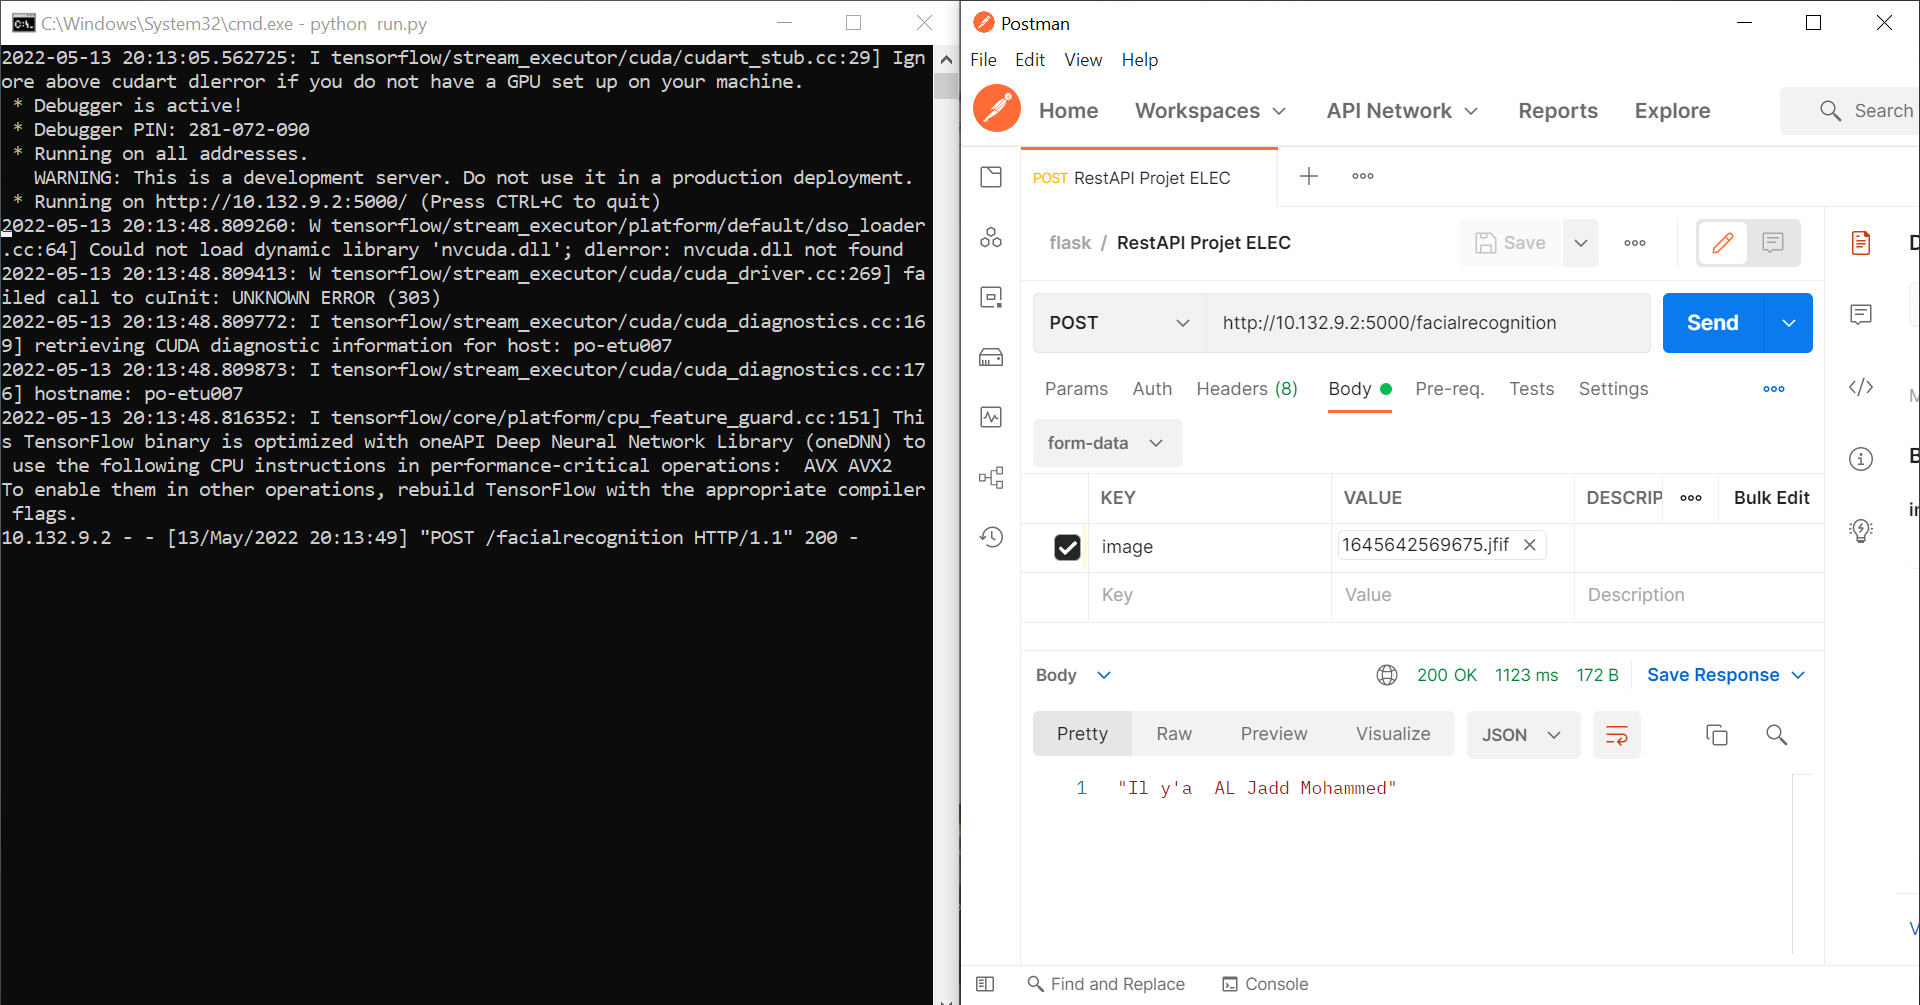
\includegraphics[width=13cm, height=6cm]{4-Images/Postman-test-api.PNG}}
\caption{Postman}
\label{fig:figure10}
\end{figure}

À gauche, côté serveur, 200 est la réponse standard pour les demandes HTTP réussies.
\href{https://en.wikipedia.org/wiki/List_of_HTTP_status_codes#200}{Lien Wikipedia (200 status code)}









% Chapter 5 Traitement video ---------------------------------------------------------
% -------------------------------------------------------------------
\pagebreak

\lhead{Mode II : Traitement video}
\section{Mode II : Traitement video}\thispagestyle{fancy}


\subsection{Sockets}
\begin{wrapfigure}[20]{r}[0.5cm]{0.3\textwidth}
\centering
\frame{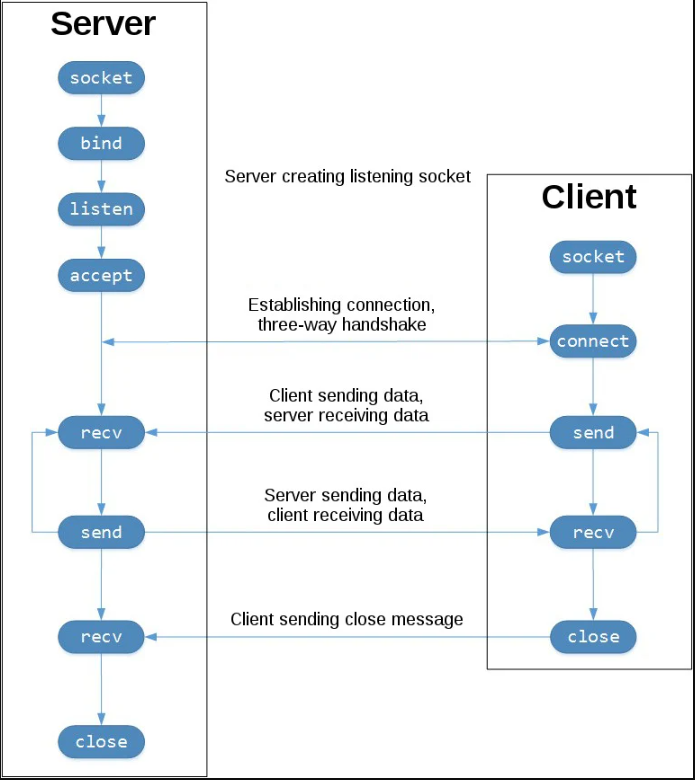
\includegraphics[width=6cm, height=6cm]{4-Images/sockets-workflow.PNG}}
\caption{Organigramme des sockets}
\label{fig:figure3}
\end{wrapfigure} 
Les socket, défini par le couple (adresse IP, numéro de port), est un point de terminaison dans une communication. Ils peuvent utiliser soit le protocol TCP ou UDP. Les étapes pour établir une communication entre le serveur et le client sont les suivantes :

\begin{itemize}
    \item 
    \item Création d'une socket (côté serveur).
    \item Bind : Affecter le couple (Addresse IP, Port) au socket (côté serveur).
    \item Listen : Attendre les connexions entrantes (côté serveur).
    \item Accept : Accepter une ou plusieurs connexions (côté serveur).
\end{itemize}

Après cela, nous pouvons envoyer et recevoir des données.



\subsection{Schéma}

\subsection{Communication bidirectionnelle}
Pour que la carte Raspberry PI puisse envoyer des données et recevoir des résultats en même temps, nous devons choisir un autre port pour la réception des données. Notez que chaque socket a son propre tuple (IP, Port). Dans l'image suivante, nous voyons clairement qu'il y a deux sockets.
\begin{figure}[H] 
\centering
\frame{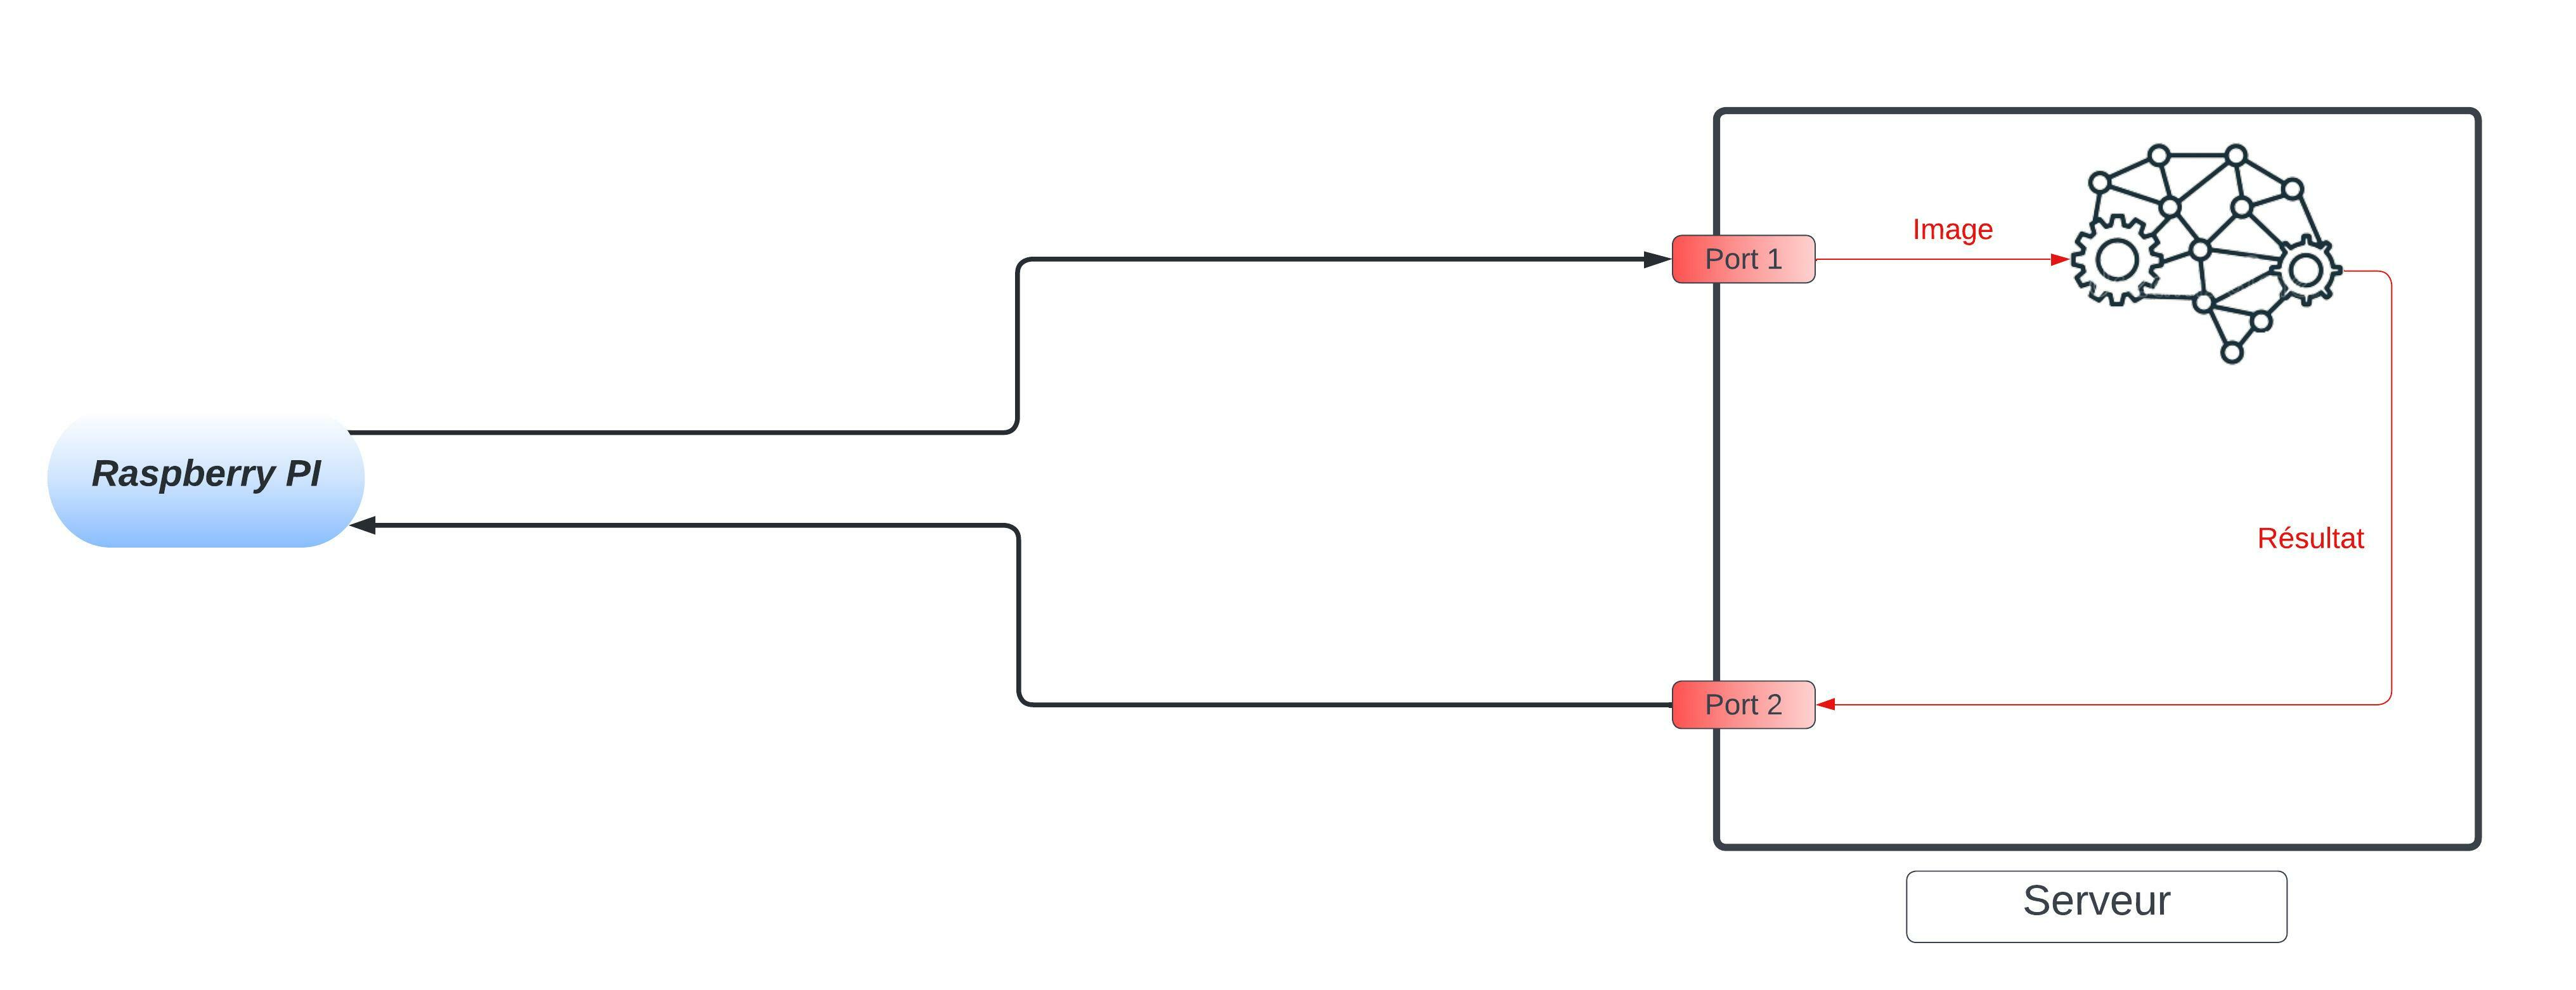
\includegraphics[width=13cm, height=5cm]{4-Images/Organigramme des sockets.jpeg}}
\caption{Communication bidirectionnelle}
\label{fig:figure10}
\end{figure}

Supposons que l'adresse IP du serveur soit 10.10.1.2 et que les deux ports soient respectivement 8001 et 8002.
\begin{center}
    \begin{itemize}
        \item Socket 1 (10.10.1.2, 8001).
        \item Socket 2 (10.10.1.2, 8002).
    \end{itemize}
\end{center}



% Chapter 6 ---------------------------------------------------------
% -------------------------------------------------------------------

\pagebreak
\lhead{Démonstration}
\chapter{Démonstration}\thispagestyle{fancy}

Comme nous avons réussi à atteindre les deux objectifs, le mode image et le mode vidéo, nous laissons le choix à l'utilisateur de décider quel mode il veut choisir. Dans l'image suivante, nous présentons comment, à l'aide de cinq boutons, l'utilisateur peut choisir un mode et ensuite un des trois services. Il peut également passer d'un mode à l'autre à tout moment. Notez que la précition de texte dans le mode vidéo ne sera pas disponible parce que nous ne voulons pas que l'utilisateur entende le même texte plusieurs fois, en particulier lorsque le texte est très long.

\begin{figure}[H] 
\centering
\frame{\adjincludegraphics[width=14cm, height=9.5cm,clip]{4-Images/ButtonFlowchart.PNG}}\\[0.5cm]
\caption{Organigramme des boutons}
\label{fig:figure17}
\end{figure}

% Chapter 5 ---------------------------------------------------------
% -------------------------------------------------------------------

\pagebreak
\lhead{Organisation}

\chapter{Organisation}\thispagestyle{fancy}
\section{Gantt}
A Gantt chart is a type of bar chart that illustrates a project schedule, named after its popularizer, Henry Gantt, who designed such a chart around the years 1910–1915. Modern Gantt charts also show the dependency relationships between activities and the current schedule status

\section{Github}
GitHub, Inc. is a provider of Internet hosting for software development and version control using Git. It offers the distributed version control and source code management functionality of Git, plus its own features

\section{Budget}
GitHub, Inc. is a provider of Internet hosting for software development and version control using Git. It offers the distributed version control and source code management functionality of Git, plus its own features


\section{Méthode de travail}
GitHub, Inc. is a provider of Internet hosting for software development and version control using Git. It offers the distributed version control and source code management functionality of Git, plus its own features

% Chapter 6 ---------------------------------------------------------
% -------------------------------------------------------------------


\pagebreak
\lhead{Code source du projet}
\chapter{Code source du projet}\thispagestyle{fancy}
Vous trouvez dans ce \href{https://github.com/mohammedAljadd/iEars}{lien} le code source de notre projet inclu les deux versions.\\

\begin{center}
\begin{figure}[H]
\centering
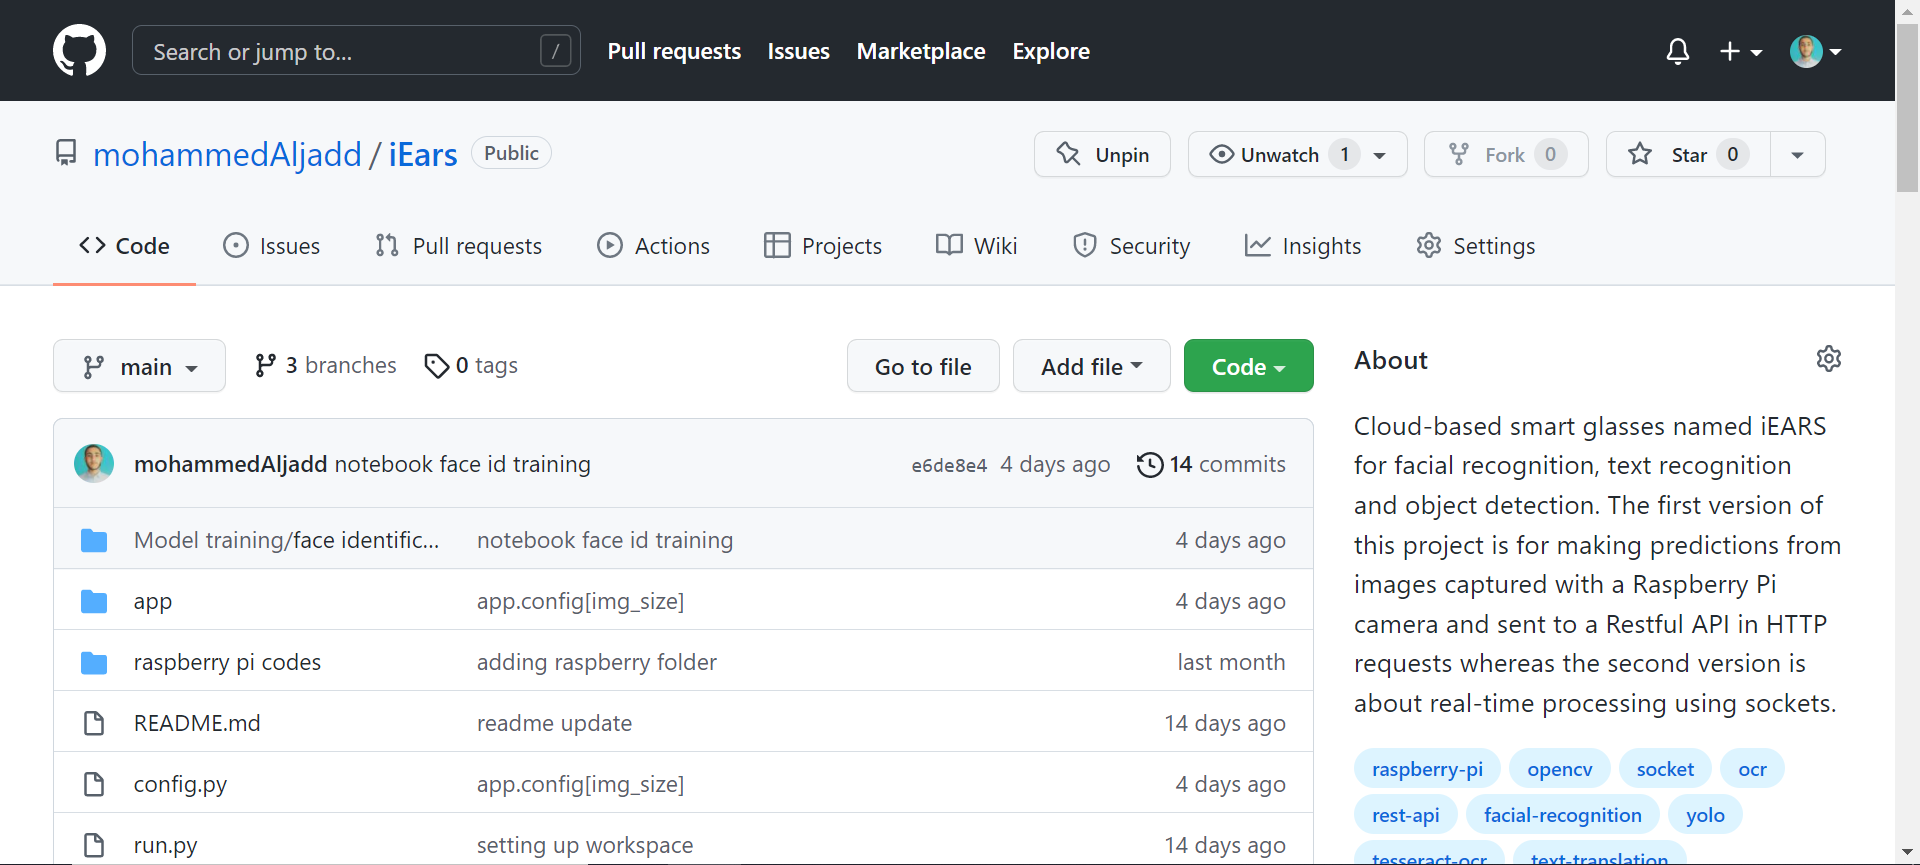
\includegraphics[width=18cm, height=7cm]{4-Images/github.PNG}\\[2cm]
\caption{Github}
\label{fig:figure11}
\end{figure}
\Large

\end{center}


% Chapter 7 ---------------------------------------------------------
% -------------------------------------------------------------------

\pagebreak
\lhead{Références}
\chapter{Références}

\textbf{\textcolor{blue}{[1]} \href{https://towardsdatascience.com/build-a-handwritten-text-recognition-system-using-tensorflow-2326a3487cd5}{Text Recognition System}}\\

\textbf{\textcolor{blue}{[2]} 
\href{ https://arxiv.org/pdf/1409.1556.pdf }{Article VGG-16}} \\

\textbf{\textcolor{blue}{[3]} \href{https://docs.python.org/3/library/socket.html}{Sockets}} \\

\textbf{\textcolor{blue}{[4]} \href{https://www.youtube.com/watch?v=GMppyAPbLYk}{RestAPI tutorial}}\\

\textbf{\textcolor{blue}{[5]} \href{https://www.mathworks.com/help/deeplearning/ref/vgg16.html}{VGG-16 expliquation}} \\


\textbf{\textcolor{blue}{[6]} \href{https://www.datacorner.fr/yolo-intro/}{Introduction to YOLO with Darknet}} \\

\textbf{\textcolor{blue}{[7]} \href{https://pjreddie.com/media/files/papers/yolo.pdf}{Article YOLO}} \\


\textbf{\textcolor{blue}{[8]} \href{https://www.aqsone.com/blog/2021/data-science-fr/comment-detecter-les-objets-plus-efficacement-avec-yolo/}{Détails sur l'aspect théorique de YOLO}} \\

\textbf{\textcolor{blue}{[9]} \href{https://blog.51cto.com/u_15435490/4632460}{Algorithme de segmentation}} \\

\textbf{\textcolor{blue}{[10]} \href{https://www.bilibili.com/video/BV1Wi4y1d7u1?spm_id_from=333.337.search-card.all.click}{Reconnaissance de texte OCR}} \\

\textbf{\textcolor{blue}{[11]} \href{https://blog.csdn.net/lin_ff/article/details/87307904?spm=1001.2101.3001.6650.5&utm_medium=distribute.pc_relevant.none-task-blog-2~default~BlogCommendFromBaidu~Rate-5-87307904-blog-108687481.pc_relevant_paycolumn_v3&depth_1-utm_source=distribute.pc_relevant.none-task-blog-2~default~BlogCommendFromBaidu~Rate-5-87307904-blog-108687481.pc_relevant_paycolumn_v3&utm_relevant_index=8
}{Algorithme de segmentation dans la reconnaissance de texte}} \\


\textbf{\textcolor{blue}{[12]} \href{https://blog.csdn.net/qq_40414818/article/details/84349232}{Segmentation des caractères chinois manuscrits}} \\


\textbf{\textcolor{blue}{[12]} \href{https://github.com/githubharald/SimpleHTR}{HTR}} \\


\textbf{\textcolor{blue}{[13]} \href{https://www.youtube.com/watch?v=oDHpqu52soI&ab_channel=deeplizard}{Fine-tune VGG16}} \\


\textbf{\textcolor{blue}{[14]} \href{https://raspberry-lab.fr/Composants/Utilisation-Camera-sur-Raspberry-Pi-Francais/}{Configuration de la caméra Raspberry Pi}} \\

\textbf{\textcolor{blue}{[15]} \href{https://raspberrypihq.com/use-a-push-button-with-raspberry-pi-gpio/
}{configuration des boutons poussoirs}} \\


\textbf{\textcolor{blue}{[16]} \href{https://raspberry-pi.fr/installer-raspbian-premier-demarrage-configuration/}{Installation du Raspbian OS}} \\


\textbf{\textcolor{blue}{[17]} \href{https://raspberry-pi.fr/connecter-ssh-raspberry-pi/}{Connexion SSH au Raspberry Pi}} \\


\textbf{\textcolor{blue}{[18]} \href{https://www.tomshardware.com/how-to/install-vnc-raspberry-pi-os}{Affichage de Rapsberry pi via VNC}} \\





